\documentclass{beamer}

%% \documentclass[handout]{beamer}
%% % use this with the [handout] option to create handouts for the audience
%% \usepackage{pgfpages}
%% \pgfpagesuselayout{2 on 1}[a4paper,border shrink=5mm]

\mode<presentation>
{
  \usetheme{Diku}
% set this to your preferences:
  \setbeamercovered{invisible}
%  \setbeamercovered{transparent}
}

\usepackage{graphicx}
\usepackage{epic}

\usepackage{amsmath}
\usepackage{amssymb}
\usepackage{amsthm}

\newcommand{\basetop}[1]{\vtop{\vskip-1ex\hbox{#1}}}
\newcommand{\source}[1]{\let\thefootnote\relax\footnotetext{\scriptsize\textcolor{kugray1}{Source: #1}}}

% for coloured code citation in text:
\usepackage{fancyvrb}

%%%%%%%%%%%%%%%%%%%%%%%%%%%%%%%%%
%%%%%    code sections   %%%%%%%%
%%%%%%%%%%%%%%%%%%%%%%%%%%%%%%%%%

% code highlighting commands in own block
\DefineVerbatimEnvironment{code}{Verbatim}{fontsize=\scriptsize}
\DefineVerbatimEnvironment{icode}{Verbatim}{fontsize=\scriptsize}

% Fancy code with color commands:
\DefineVerbatimEnvironment{colorcode}%
        {Verbatim}{fontsize=\scriptsize,commandchars=\\\{\}}

%%%%%%%%%%%%%%%%%%%%%%%%%%%%%%%%%%
%%%%%    some coloring    %%%%%%%%

\definecolor{Red}{RGB}{220,50,10}
\definecolor{Blue}{RGB}{0,51,102}
\definecolor{Yellow}{RGB}{102,51,0}
\definecolor{Orange}{RGB}{178,36,36}
\definecolor{Grey}{RGB}{180,180,180}
\definecolor{Green}{RGB}{20,120,20}
\definecolor{Purple}{RGB}{160,50,100}
\newcommand{\red}[1]{\textcolor{Red}{{#1}}}
\newcommand{\blue}[1]{\textcolor{Blue}{{#1}}}
\newcommand{\yellow}[1]{\textcolor{Yellow}{{#1}}}
\newcommand{\orange}[1]{\textcolor{Orange}{{#1}}}
\newcommand{\grey}[1]{\textcolor{Grey}{{#1}}}
\newcommand{\green}[1]{\textcolor{Green}{{#1}}}
\newcommand{\purple}[1]{\textcolor{Purple}{{#1}}}




% use "DIKU green" from our color theme for \emph
\renewcommand{\emph}[1]{\textcolor{structure}{#1}}
% use some not-too-bright red for an \emp command
\definecolor{DikuRed}{RGB}{130,50,32}
\newcommand{\emp}[1]{\textcolor{DikuRed}{ #1}}
\definecolor{CosGreen}{RGB}{10,100,70}
\newcommand{\emphh}[1]{\textcolor{CosGreen}{ #1}}
\definecolor{CosBlue}{RGB}{55,111,122}
\newcommand{\emphb}[1]{\textcolor{CosBlue}{ #1}}
\definecolor{CosRed}{RGB}{253,1,1}
\newcommand{\empr}[1]{\textcolor{CosRed}{ #1}}

\newcommand{\mymath}[1]{$ #1 $}
\newcommand{\myindx}[1]{_{#1}}
\newcommand{\myindu}[1]{^{#1}}

\newcommand{\Fasto}{\textsc{Fasto}\xspace}


%%%%%%%%%%%%%%%%%%%%

\title[Interconnect]{Scalable Cache Coherence \&\\Interconnection Networks}

\author[C.~Oancea]{Cosmin E. Oancea {\tt cosmin.oancea@diku.dk}}

\institute{Department of Computer Science (DIKU)\\University of Copenhagen}


\date[Sept 2014]{September 2014 PMPH Lecture Notes}


\begin{document}

\titleslide

\begin{frame}
\frametitle{Structure of a Compiler}

\begin{tabular}{ccc}
Program text&&\\
$\downarrow$ &&\\
\framebox{Lexical analysis} && Binary machine code\\
$\downarrow$ && $\uparrow$ \\
Symbol sequence && \textcolor{gray}{\framebox{Assembly and linking}} \\
$\downarrow$ && $\uparrow$ \\
\framebox{Syntax analysis} && Ditto with named registers\\
$\downarrow$ && $\uparrow$ \\
Syntax tree && \framebox{Register allocation} \\
$\downarrow$ && $\uparrow$ \\
\red{\framebox{Type Checking}} && Symbolic machine code\\
$\downarrow$ &&  $\uparrow$ \\
Syntax tree  && \framebox{Machine code generation} \\
$\downarrow$ && $\uparrow$ \\
\framebox{Intermediate code generation} &$\longrightarrow$ & Intermediate code
\end{tabular}

\end{frame}



%%%%%%%%%%%%%%%%%%%%%%%%%%%%%%%%%%%%%%%%%%%%%%%%%%%%%%%%%%%%%%%%%%%%%%
%%%%%%%%%%%%%%%%%%%%%%%%%%%%%%%%%%%%%%%%%%%%%%%%%%%%%%%%%%%%%%%%%%%%%%
%%%%%%%%%%%%%%%%%%%%%%%%%%%%%%%%%%%%%%%%%%%%%%%%%%%%%%%%%%%%%%%%%%%%%%
\begin{frame}[fragile]
	\tableofcontents
\end{frame}

%%%%%%%%%%%%%%%%%%%%%%%%%%%%%%%%%%%%%%%%%%%%%%%%%%%
%%%%%%%%%%%%%%%%%%%%%%%%%%%%%%%%%%%%%%%%%%%%%%%%%%%
%%%%%%%%%%%%%%%%%%%%%%%%%%%%%%%%%%%%%%%%%%%%%%%%%%%

\section{Scalable Shared Memory Systems}

\begin{frame}[fragile,t]
\frametitle{Bus-Based SMPs Do Not Scale}

\emph{Ideally, memory bandwidth should scale linearly with the number of nodes,
and memory latency should remain constant}.\bigskip

\alert{Bus-Based Multiprocessors are inherently NON-Scalable}:\medskip
\begin{itemize}
    \item \emp{Bus Bandwidth} capped by {\tt (\# of bus wires)$\times$clockrate}, and
    \item \emp{actually decreases as more noded are added}, 
            because the wire length and the load on them 
            increases with the number of nodes.\bigskip
    \item Dance Hall: memory latency about the same for any access,
            but as the \# of procs goes up, the latency of all
            accesses increases.\bigskip
    \item \emp{Snoopy (Broadcast) Based Protocols are NOT Scalable},
            because involve {\em all} nodes in {\em all} coherence transactions. 
\end  {itemize}
\end{frame}

\begin{frame}[fragile,t]
\frametitle{cc-NUMA: Cache Coherent Non-Uniform Mem Arch}

\emph{Def. Scalable: memory bandwidth should grows linearly and
memory access latency grows sub-linearly with the number of nodes}.
%\vspace{-5ex}
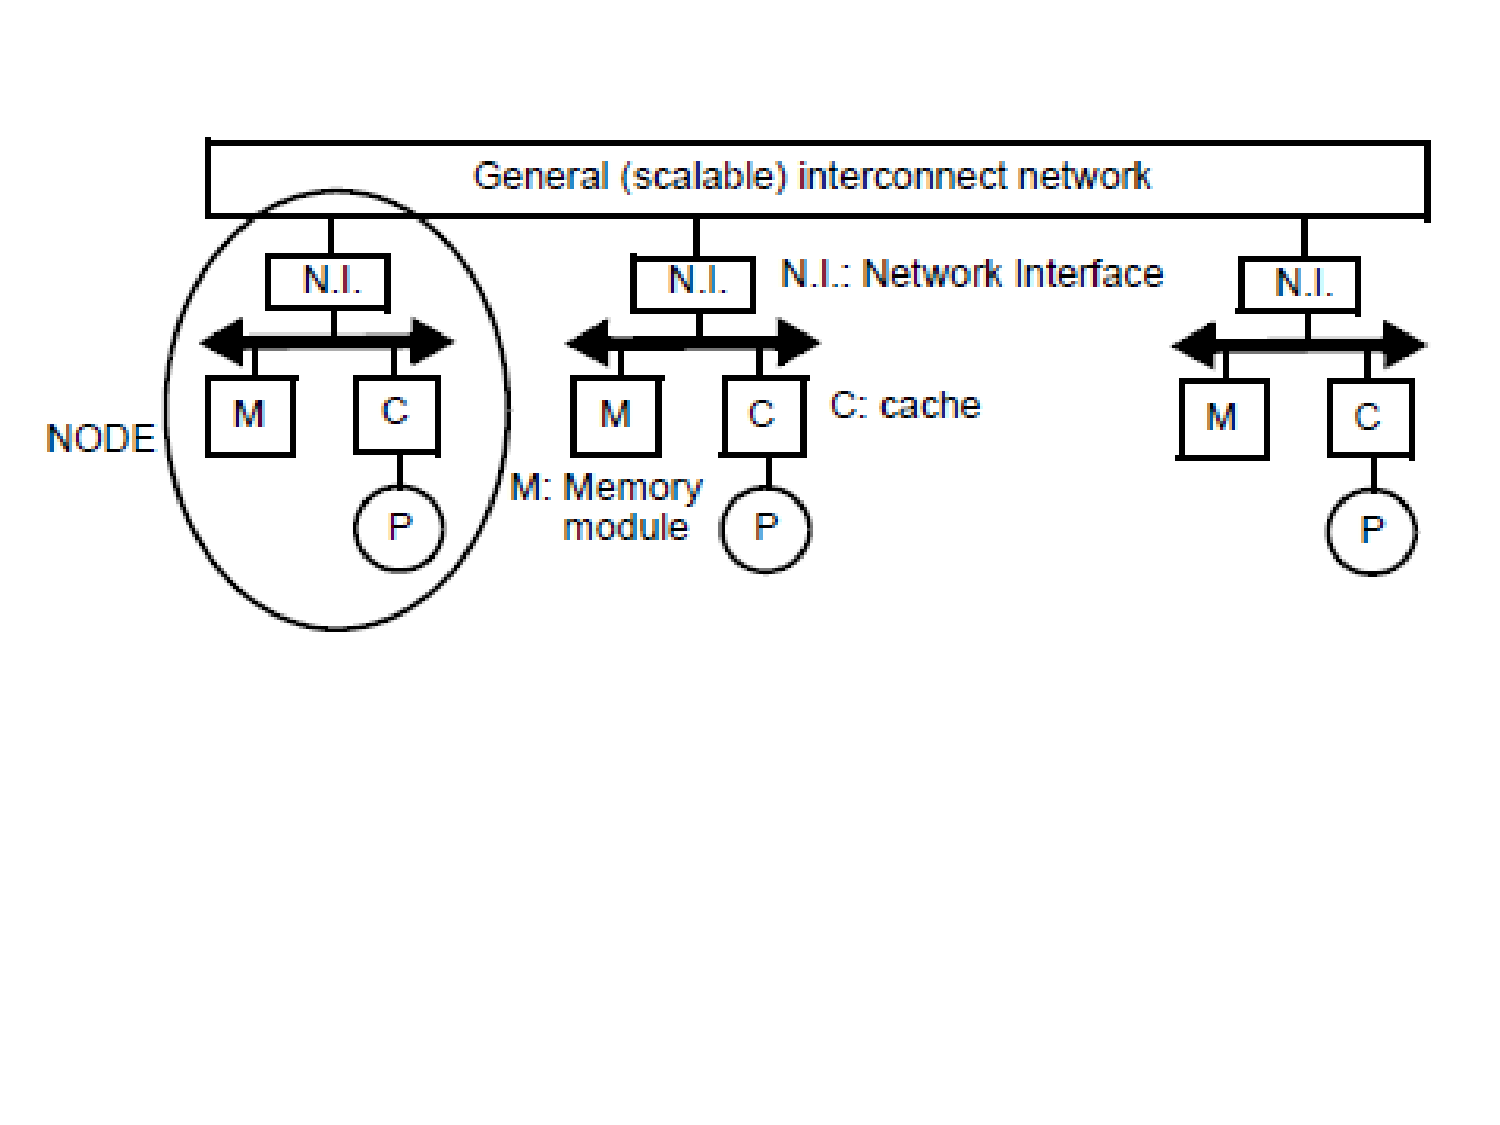
\includegraphics[width=59ex]{FigsInfCoherence/MultiNode}
\vspace{-20ex}

\emph{cc-NUMA} because latency of a local mem module is $<$ of a remote:\\
\begin{itemize}
    \item Memory partitioned into banks \& distributed across nodes 
            to leverage locality. Can be Main Mem or shared cache (NUCA).
    \item Uses a scalable interconnect to accomodate bandwidth,
    \item \emph{Uses scalable directory protocols to keep track of sharing.}
\end  {itemize}

\end{frame}

\begin{frame}[fragile,t]
\frametitle{Hardware Structure for Baseline Directory Protocol}

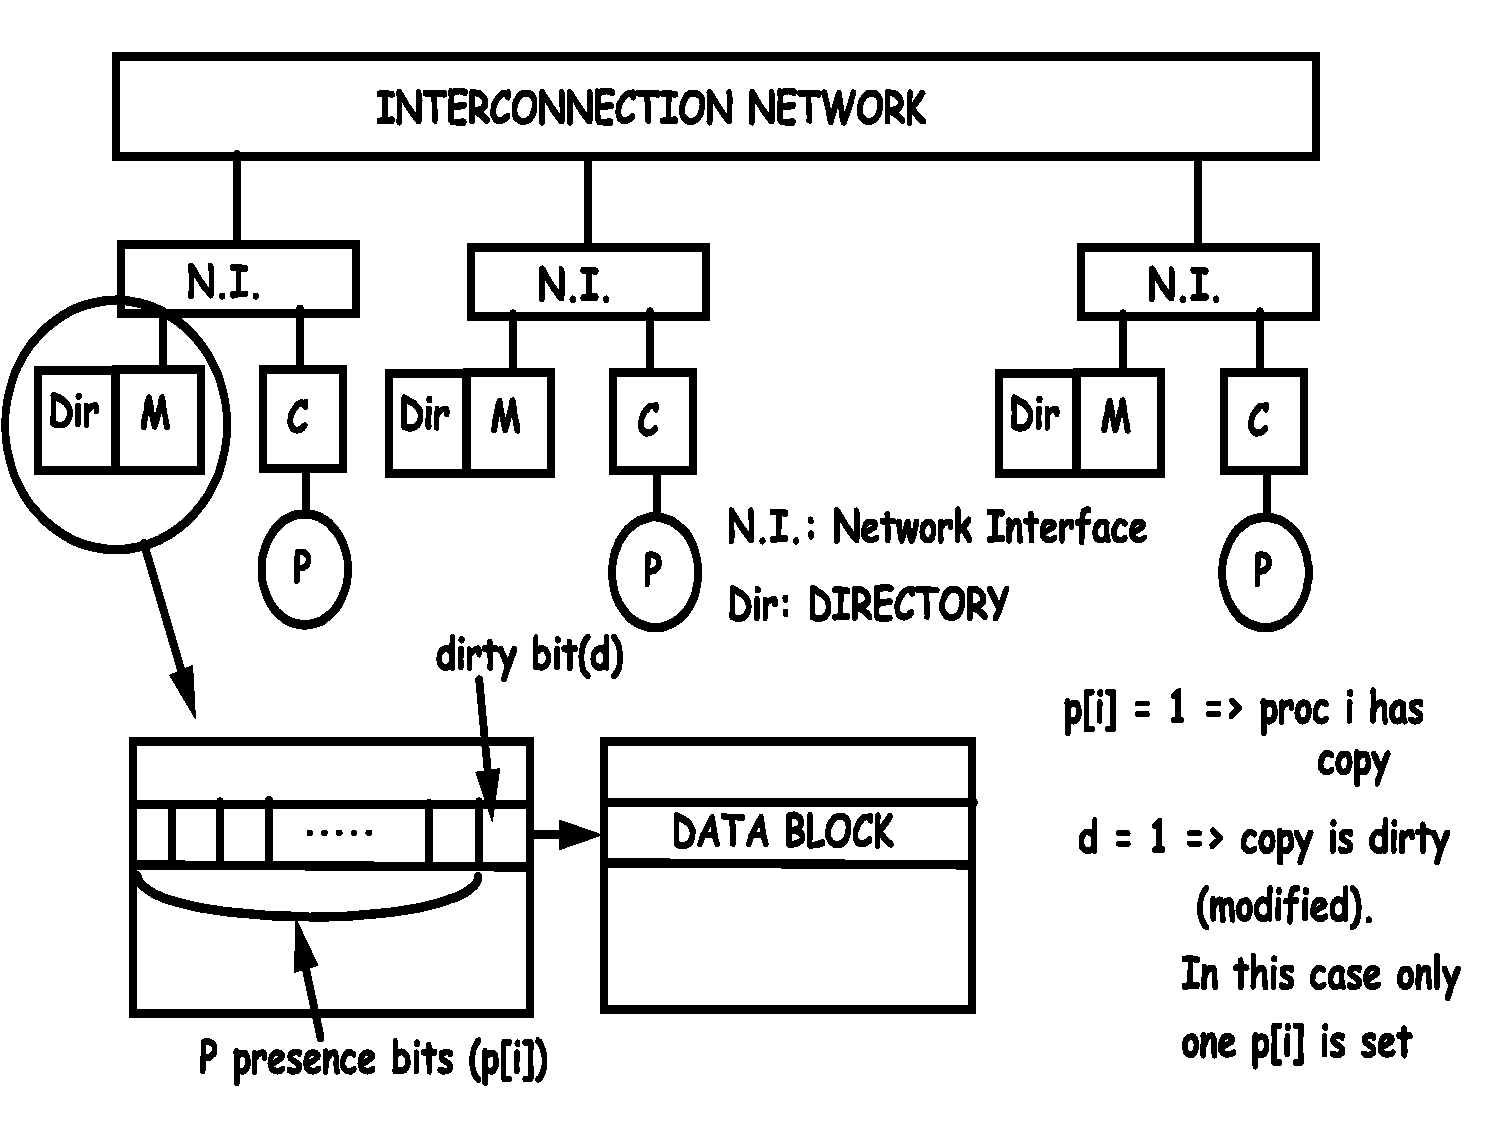
\includegraphics[width=59ex]{FigsInfCoherence/DirBasedProt}

\end{frame}

\begin{frame}[fragile,t]
\frametitle{Presence-Flag Vector Scheme}

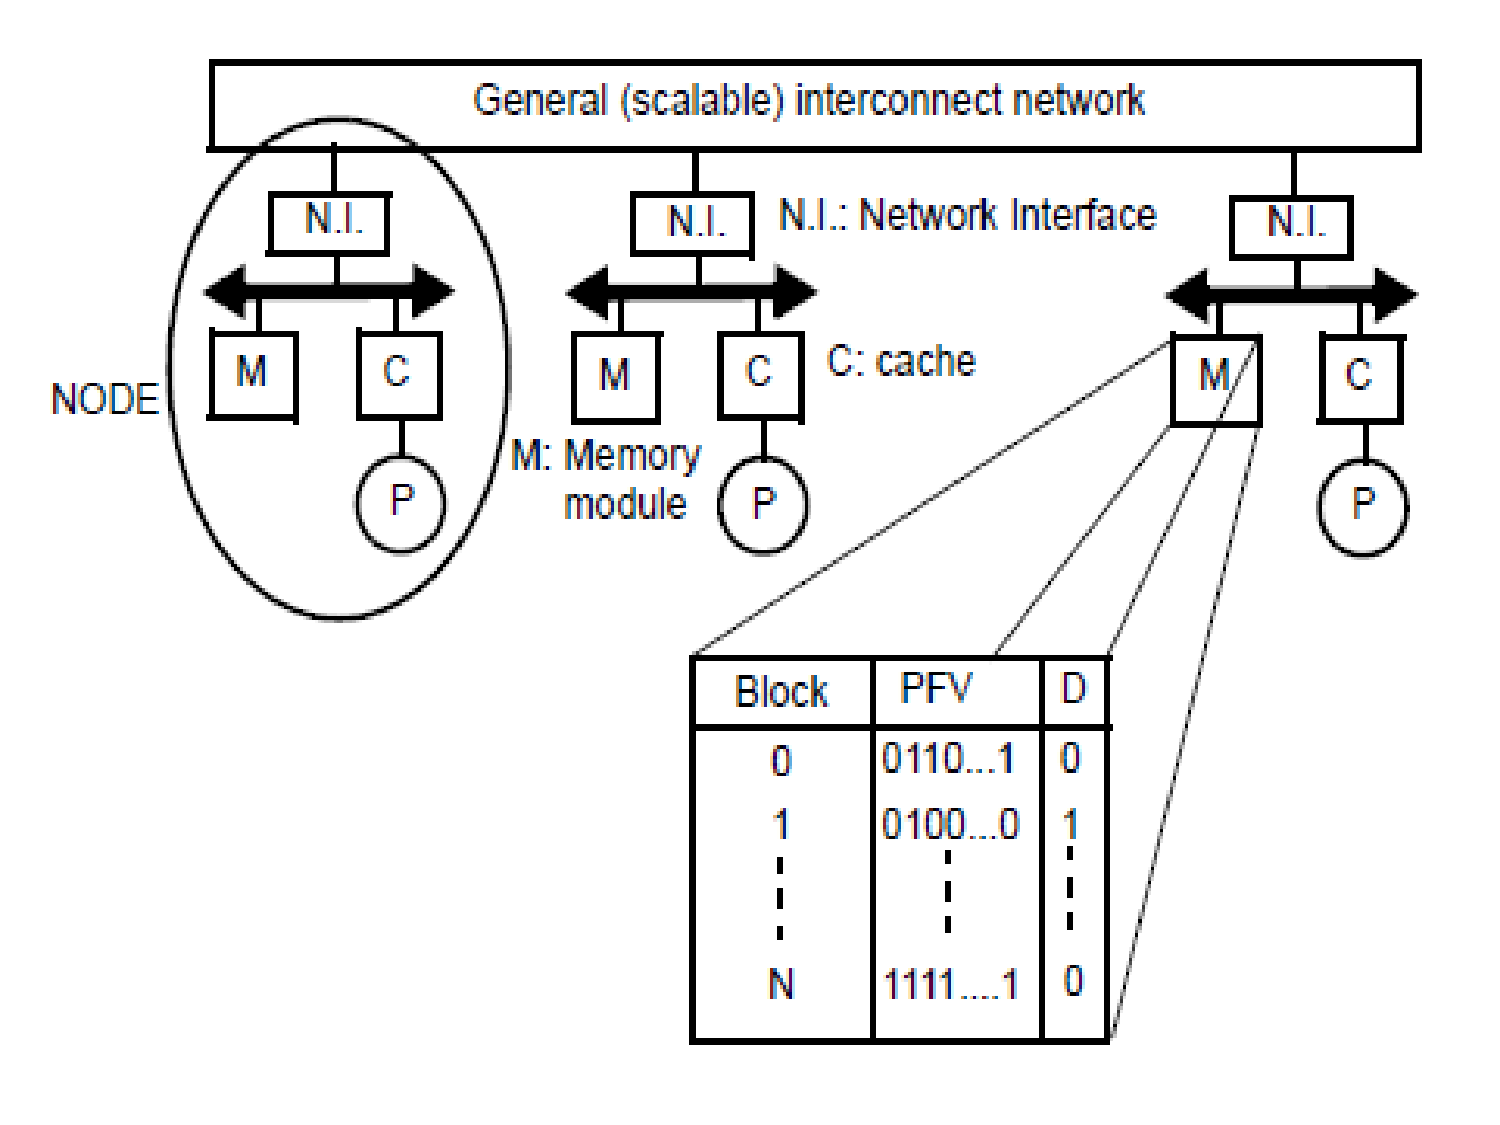
\includegraphics[width=48ex]{FigsInfCoherence/PresenceFlag}
\vspace{-2ex}

A memory block can be in two states: Clean or Dirty. Example:
\begin{itemize}
    \item Block 1 is cached by processor 2 only and is \emp{Dirty},
            i.e., memory is stale and the only valid copy is at a remote node.
    \item Block N is cached by all procs and is \emph{Clean} (mem is up to date).
\end  {itemize}

\end{frame}

\begin{frame}[fragile,t]
\frametitle{cc-NUMA Protocols}

Protocol is similar to MSI-Invalidate (or MSI-Update or MESI),
but without broadcast.
Instead uses only the (protocol) agents:
\begin{itemize}
    \item \emph{Home Node (H)} is the node where the memory block and its 
            directory entry reside,
    \item \emph{Local Node (L)} or requester is the node initiating the request,
    \item \emp{Remote Node (R)} is any other node participating in transaction:
        \begin{itemize}
            \item \emp{Dirty Node (D)} is the node holding the latest modified copy,
            \item \emp{Shared Nodes (S)} are the nodes holding a shared copy. 
        \end  {itemize}
    \item Home may be the same as Local or Dirty.
\end  {itemize}

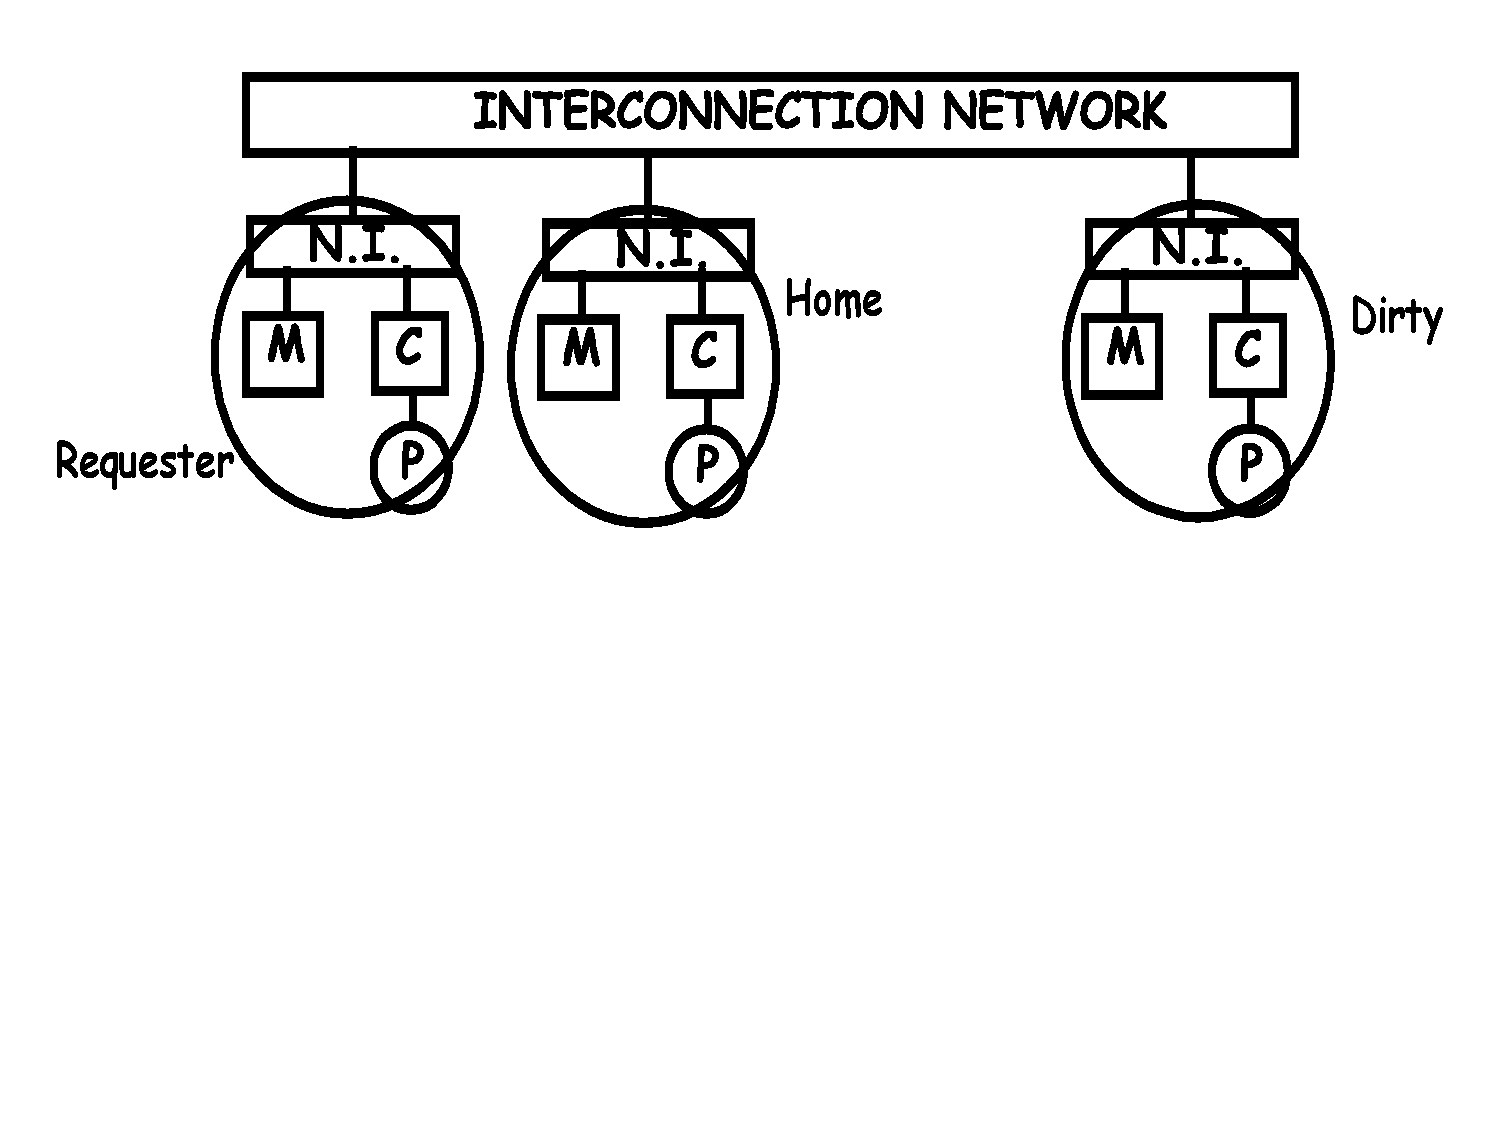
\includegraphics[width=55ex]{FigsInfCoherence/ccNUMA}
\vspace{-1ex}

A block copy can be in two states: Clean or Dirty. Example:
\begin{itemize}
    \item Block 1 is cached by processor 2 only and is Dirty
    \item Block N is cached by all processors and is Clean.
\end  {itemize}

\end{frame}

\begin{frame}[fragile,t]
\frametitle{MSI Invalidate in ccNUMA}

\begin{columns}
\column{0.66\textwidth}
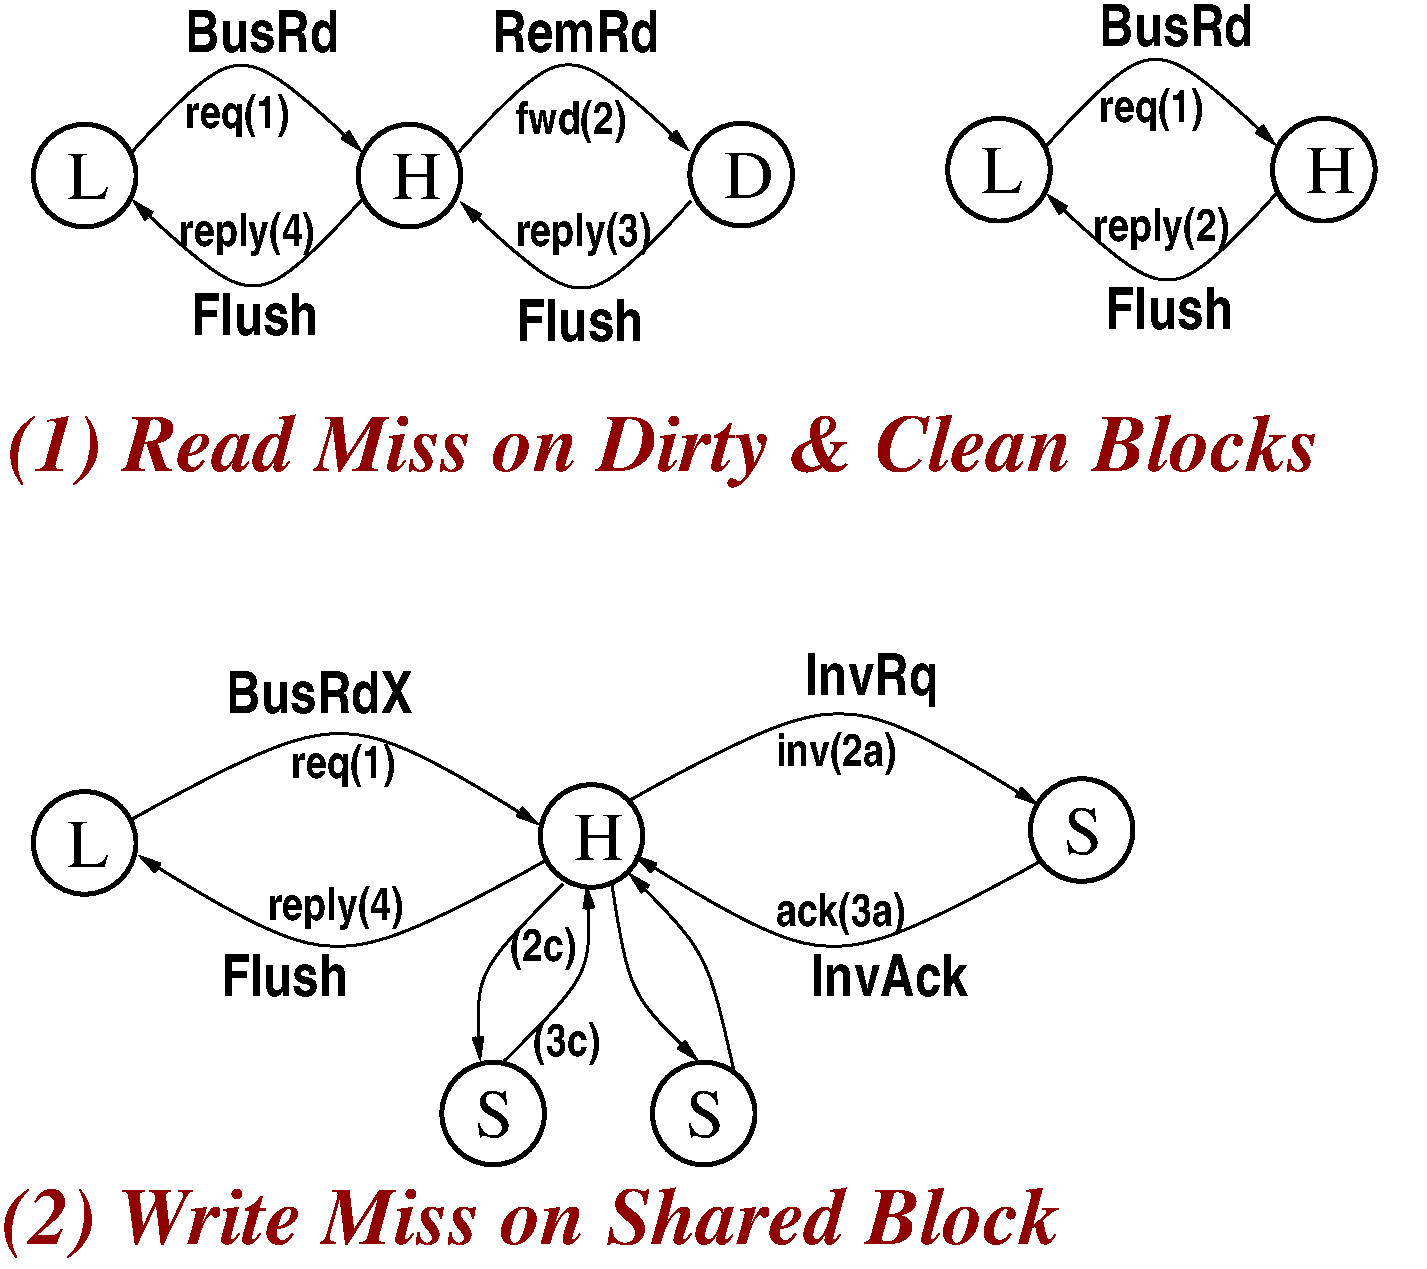
\includegraphics[width=45ex]{FigsInfCoherence/MSIccNUMA}\pause
\column{0.46\textwidth}
\begin{scriptsize}
\begin{itemize}
    \item \emp{Read Miss on Dirty Block:} local node send {\em bus-read} request to host 
                $\Rightarrow$ Since memory (host) is stale,
                   host sends {\em remote-read} request to dirty node, i.e., the only one 
                    set in PFV entry $\Rightarrow$ D sends copy to H $\Rightarrow$ H updates
                    memory and PFV, and sends copy to local (4 hops). 

    \item \emp{Read Miss on Clean Block:} H sends its valid copy to L (2 hops).\smallskip

    \item \emp{Write Miss on Shared Block:} L signals H
            $\Rightarrow$ H sends {\em invalidations} to all sharing nodes
            (found in {\tt PFV}) $\Rightarrow$ When host receives the acks from all 
            S nodes it updates {\tt PFV} (clears all but dirty L) and flushes block to L.
            (4 hops if parallel invs).
    \item \emp{Write Miss on Dirty Block:} dirty node flushes value to L via H.
\end  {itemize}
\end{scriptsize}
\end{columns}
\end{frame}

\begin{frame}[fragile,t]
\frametitle{Block Eviction \& Race Conditions}

\emp{When a block is evicted upon replacement}:
\begin{itemize}
    \item If dirty then OK, i.e., H automatically notified
            by L's write-back.
    \item If no dirty then silent eviction is still correct,
            but affects perform:\\ 
            \emp{Tradeoff} between the overhead of keeping 
            PFV accurate and the overhead of processing 
            useless invalidations.    
\end  {itemize}
\bigskip

Race Conditions: same-block transactions \emp{must not interleave}. \alert{How?}\pause
\begin{itemize}
    \item[1] Home node is the \emph{central arbiter.}
    \item[2] Use a \emph{lock bit per entry} to signal in-progress transaction.
    \item[3] If block-bit set and another transaction then:\\
                \emph{Queueing incomming requests until buffer full then NACK} $\Rightarrow$\\
                reduced latency and bandwidth and simple overflow treatment.
\end  {itemize}
\bigskip

\alert{When should the Lock Bit be cleared/turned off?}
\end{frame}


\begin{frame}[fragile,t]
\frametitle{When to Turn Off the Lock Bit?}

\begin{columns}
\column{0.66\textwidth}
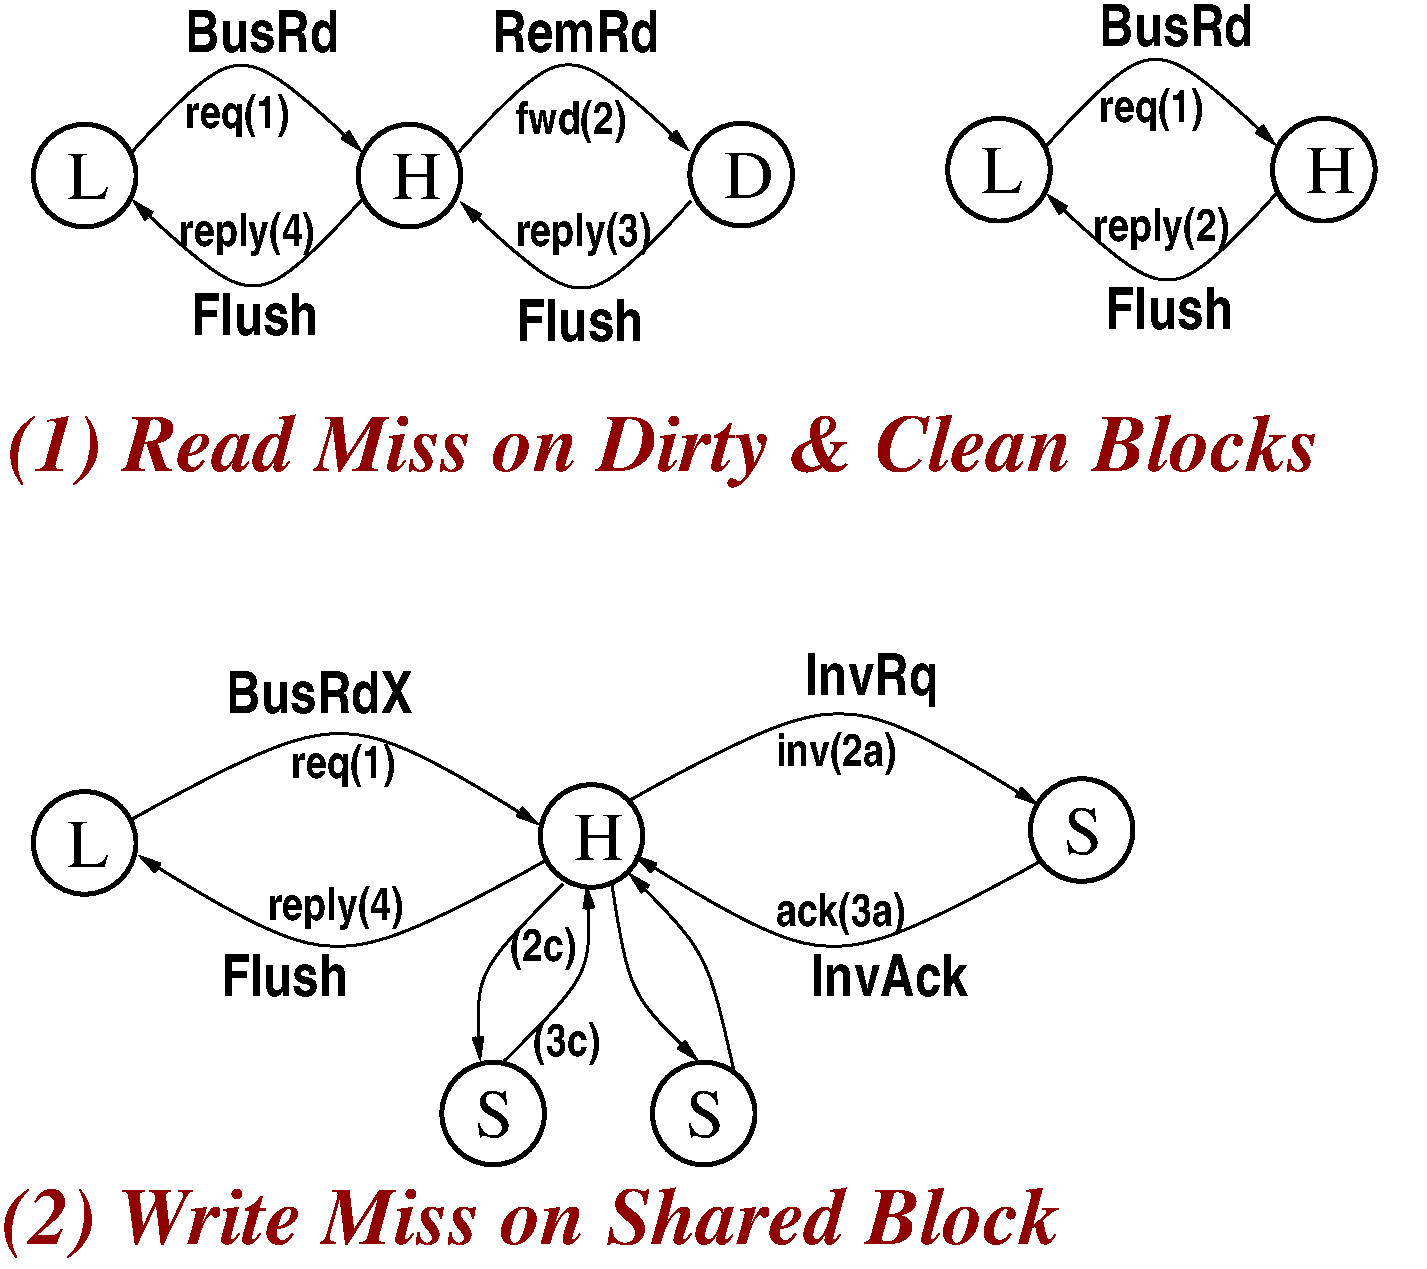
\includegraphics[width=45ex]{FigsInfCoherence/MSIccNUMA}
\column{0.46\textwidth}
Example using Fig \emp{(2)} then \emp{(1)}:
\begin{scriptsize}
\begin{itemize}
    \item The latest time the lock bit can be turned off is
            just before H {\tt Flush}es to L. \alert{Not good enough:}\pause
    \item L is now marked dirty. Assume H receives a read request on 
            the same block and forwards it to L, which is now the 
            dirty node.
    \item If {\tt RemRd} reaches L before the {\tt Flush} from H Then \alert{failure}
            because L does not have the copy yet.  
\end  {itemize}
\end{scriptsize}
\bigskip
\emph{A Solution:} L acknowledges to H the end of transaction,
        i.e., that it has received the {\tt Flush}. After
        acknowledgement H can safely turn off the Lock Bit! 
\end{columns}

\end{frame}


\begin{frame}[fragile,t]
\frametitle{Standard DASH System: Optimizing Latencies}

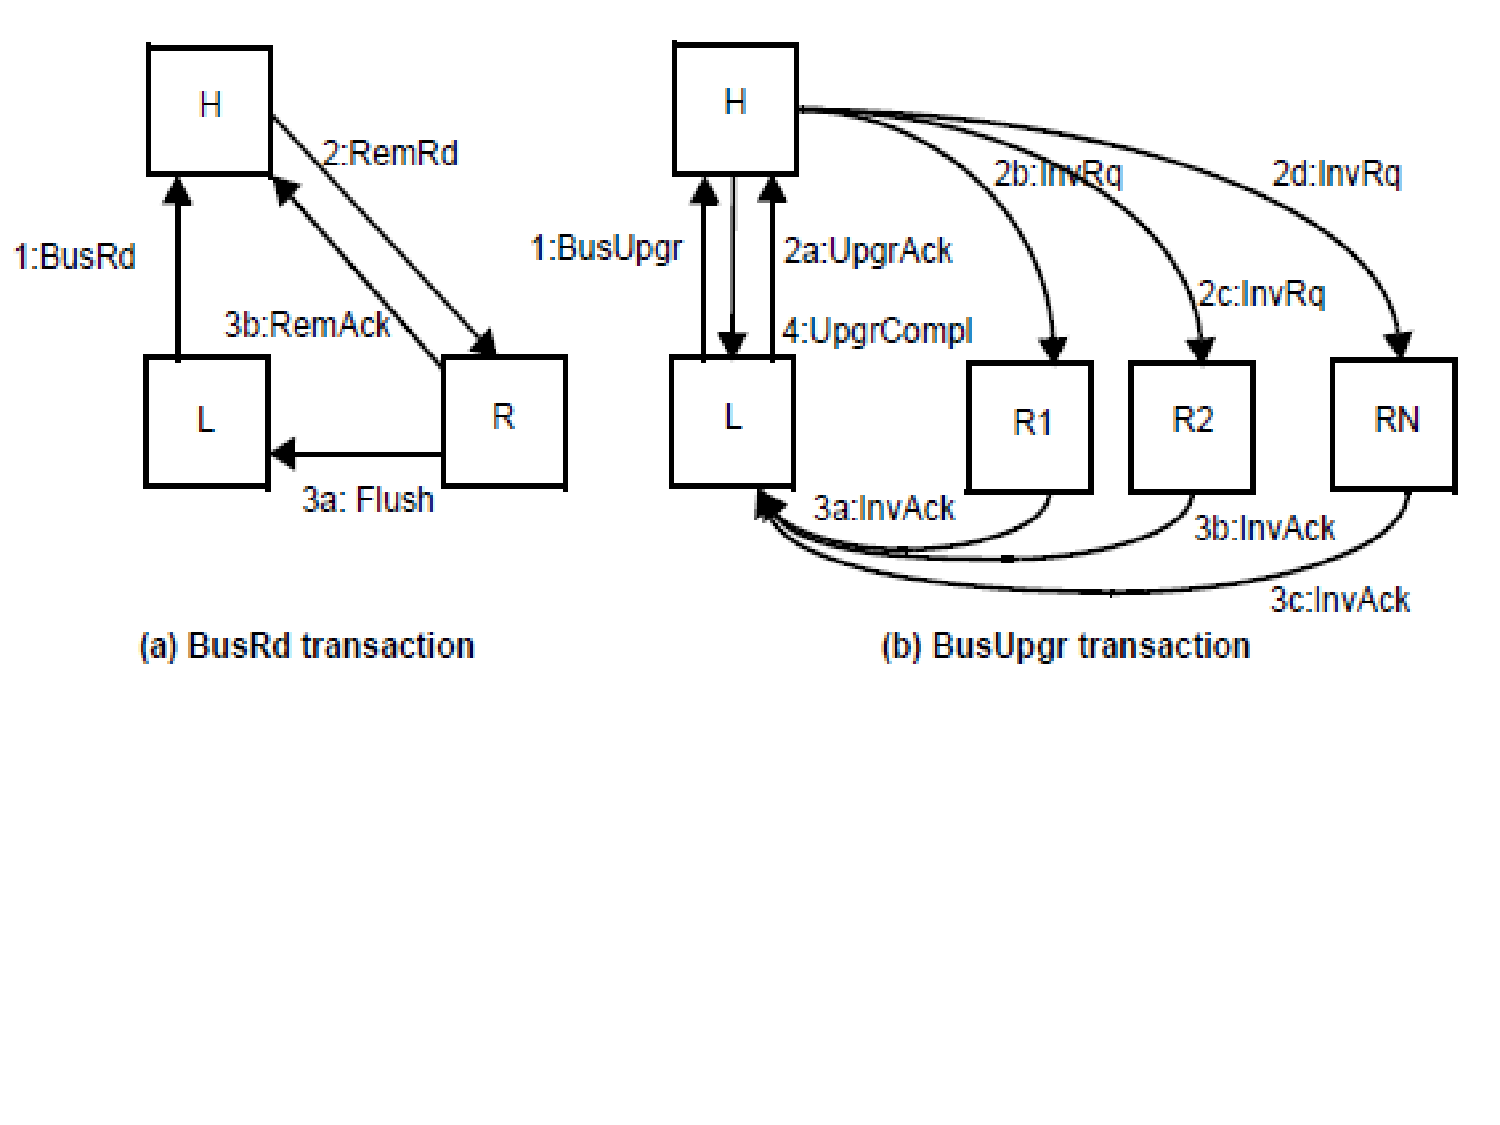
\includegraphics[width=55ex]{FigsInfCoherence/RedLatencyCCNUMA}
\vspace{-15ex}

Baseline Protocol needs at worst 4 hops. 
\emph{Can make it in THREE}:\pause
\begin{itemize}
    \item[1] Request is sent to Home
    \item[2] H redirects request to remote nodes.\\ 
             In (b) H also sends L the \# of remotes via {\tt 2a:UpgrAck}
    \item[3] Remote responds to L (L now knows when all have responded).\medskip
    \item[4] L notifies transaction completed, \emp{off the critical access path}
\end  {itemize}

\end{frame}

\begin{frame}[fragile,t]
\frametitle{Memory Requirements of Directory Protocols}

Assume $N$ nodes (processors), and $M$ memory blocks per node.
\bigskip


\emp{Total Presence-Flag Vector (PFV) Directory Size:} $M\times N\times$\alert{$N$}\\
\alert{grows linearly with N, hence a serious scalability concern.}\\
($N$ node directories, each with $M$ entries, and each entry has $N$ bits.)
\bigskip

One Alternative is Limited Pointer Protocol (LPP):
\begin{itemize}
    \item Each entry maintains $i$ pointers, each represented on {\tt log $N$} bits\\
            (instead of $N$ bits in PFV).
    \item \emp{Total LPP Directory Size:} $M\times N\times i \times$\emph{$log N$}\\ 
            \emph{grows logarithmically (sublinearly) with N} (because $i$ is constant) 
    \item Failback: resort to broadcast when the directory pointers are exhausted.
\end  {itemize}

\end{frame}


\begin{frame}[fragile,t]
\frametitle{Other Scalable Protocols}

\emp{Coarse Vector Schemes:} presence flags identify groups rather than individual nodes.
\smallskip

\emp{Directory Cache}, i.e., at cache rather than main memory level $\Rightarrow$
memory overhead is proportional to cache size (leverages locality).\medskip 

\emp{Cache-Centric Directories, for example Scalable Coherent Interface:}

\begin{columns}
\column{0.58\textwidth}
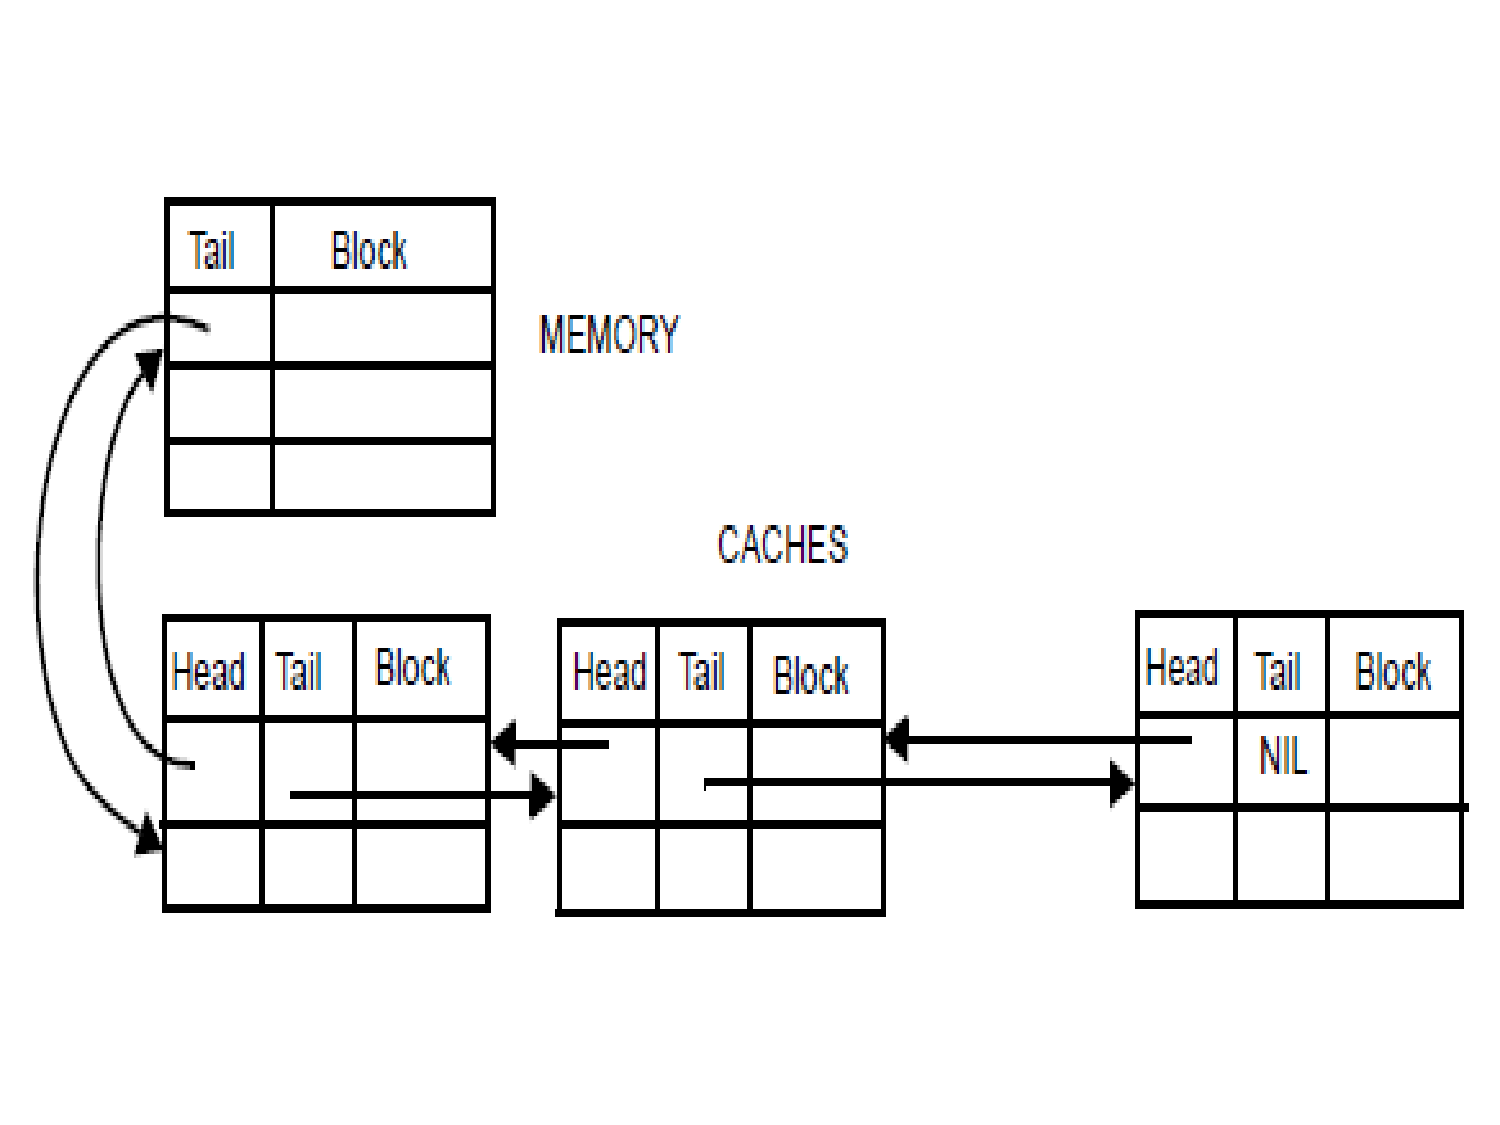
\includegraphics[width=40ex]{FigsInfCoherence/CacheCentricProt}
\column{0.48\textwidth}
\begin{scriptsize}
\begin{itemize}
    \item Directory Entry: Copies of the same memory block in different (private) 
            caches are linked via a double-linked list (implemented in cache-hardware)
    \item  \emph{Directory size proportional with the total (private) cache size},
            rather than to the main memory size as in PFV.
    \item \emp{Latency of {\tt BusRdX/BusUpgr} larger} than PFV because invalidations do not
            go in parallel (list requires sequential traversal).
    \item Bandwidth is comparable to PFV.
\end  {itemize}
\end{scriptsize}
\end{columns}

\end{frame}


\begin{frame}[fragile,t]
\frametitle{Hierarchical Systems}

\vspace{-7ex}
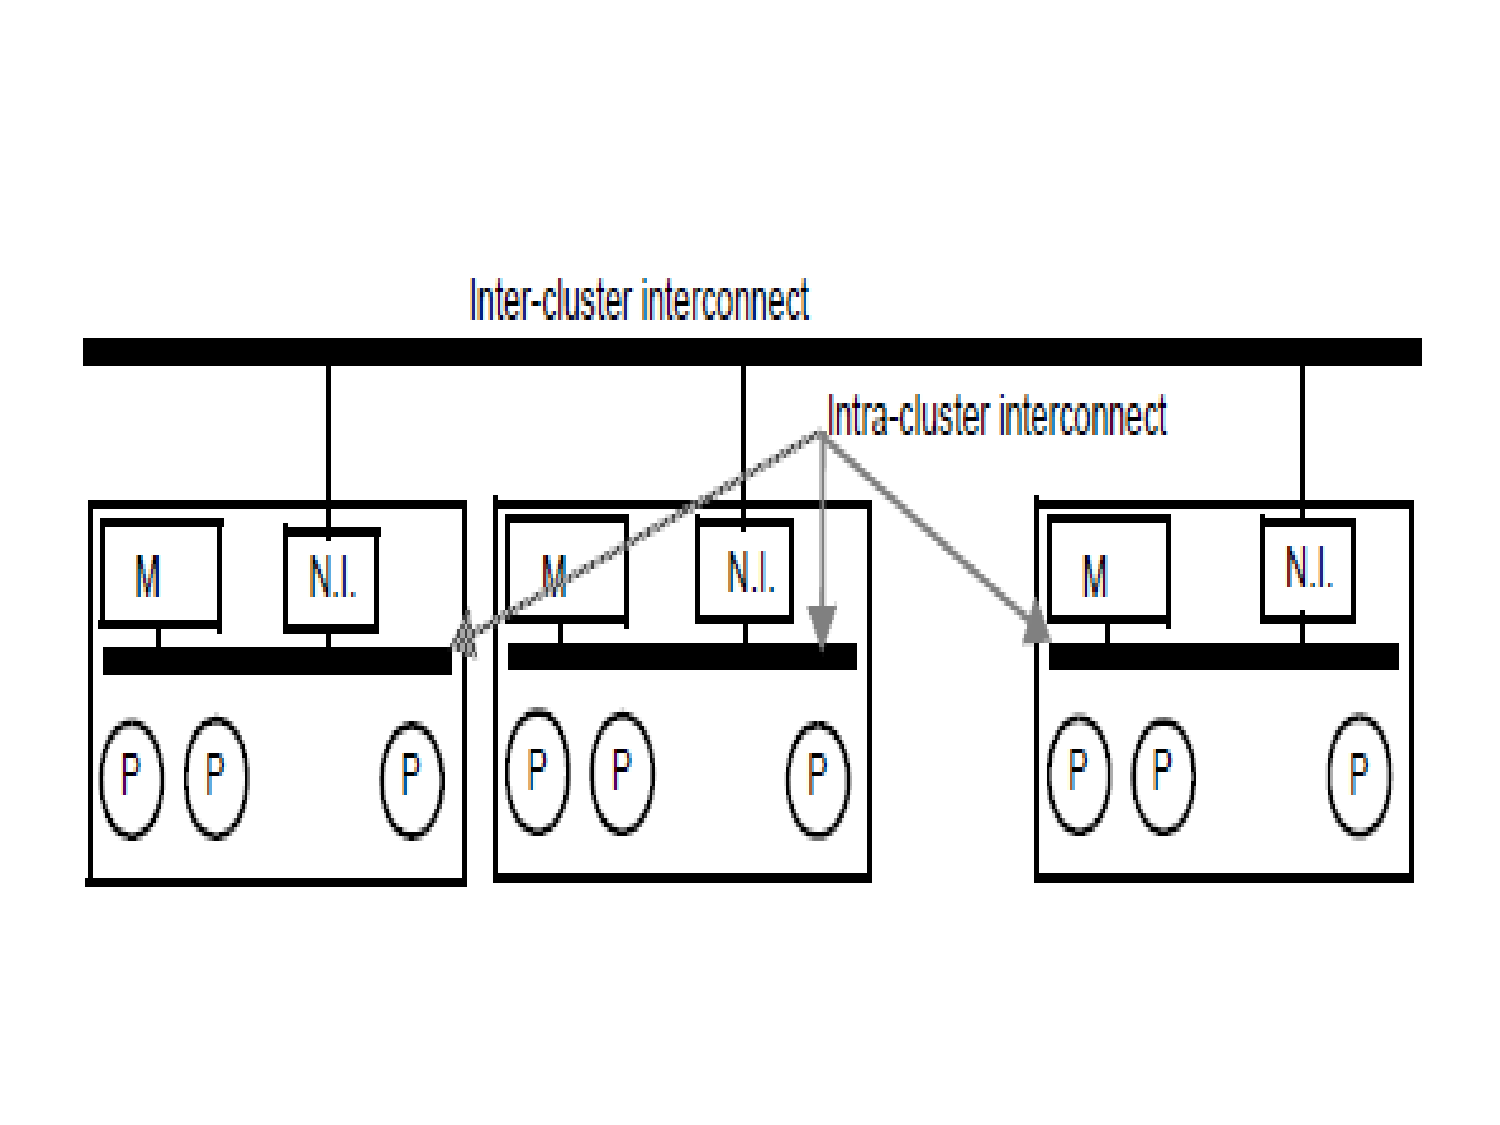
\includegraphics[width=44ex]{FigsInfCoherence/HierarchSys}
\vspace{-5ex}

Instead of scaling in a flat configuration, one can form clusters
in a hierarchical organization.   This also reduces memory overhead.\\  
Relevant inside, as well as across chip multiprocs!
\bigskip

\emp{Coherence Options:}
\begin{itemize}
    \item Intra-Cluster Coherence: snoopy / directory
    \item Inter-Cluster Coherence: snoopy / directory
    \item \alert{Tradeoffs} between memory overhead and performance to maintain coherence.
\end  {itemize}
\end{frame}


\section{Interconnection Networks (IN)}

\subsection{Design Space, Hardware Components, Communication Models}

\begin{frame}[fragile]
	\tableofcontents[currentsection]
\end{frame}

\begin{frame}[fragile,t]
\frametitle{Parallel Computer Systems}

\emp{Interconnect Networks (IN)}: 
Bringing data with low latency and high bandwidth (throughput) is paramount.
%from mem to procs 


\begin{columns}
\column{0.66\textwidth}
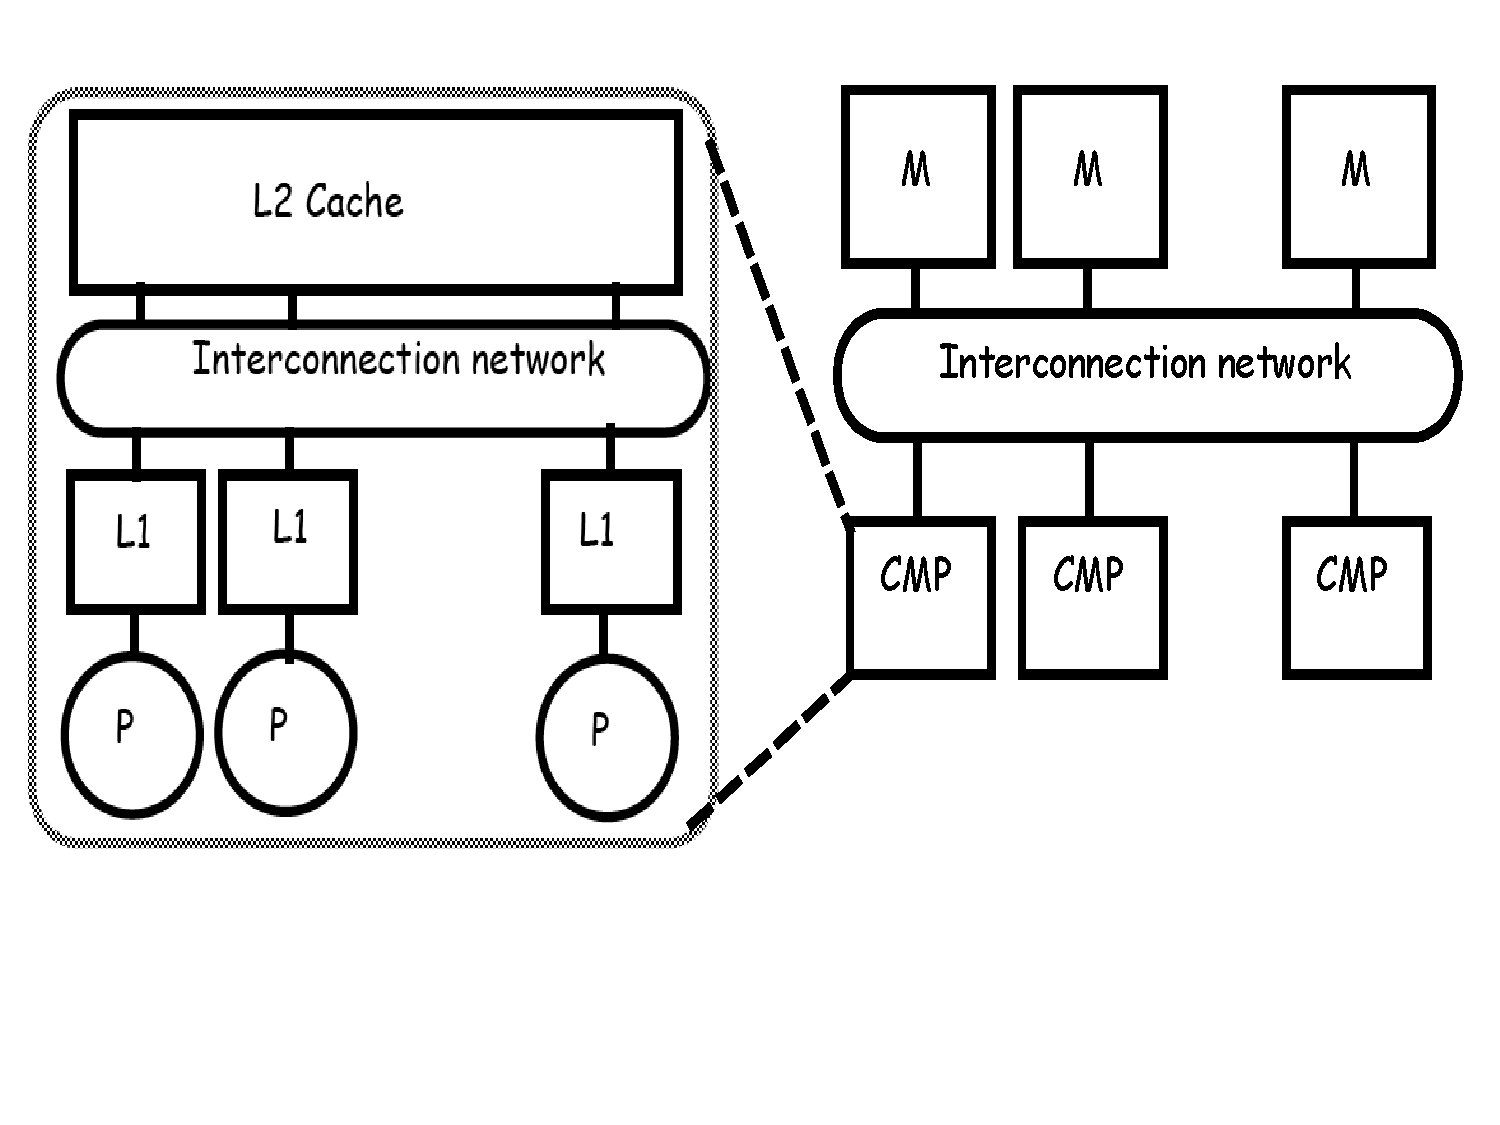
\includegraphics[width=44ex]{FigsInterconnect/ParSys}\pause
\column{0.46\textwidth}
\vspace{-6ex}
\begin{scriptsize}
\begin{itemize}
    \item \emp{IN between cores on each chip ({\sc ocn}/{\sc noc})}. 
            Shared cache bandwidth increased by splitting  
                    cache into into banks, 
                each connected to IN via a port.
            \emph{Important that IN bandwidth matches shared-cache bandwidth}
    \item \emp{IN between processor chips {\sc san}.}
            Connects chips to MM (same $\uparrow$).
            {\sc lan}/{\sc wan} not studied: similar issues,
            but different tradeoffs,\\e.g., latency not critical.
\end  {itemize}
\end{scriptsize}
\end{columns}
\vspace{-4ex}

\alert{Problem}: meeting interconnection bandwidth and latency requirement
within cost, e.g., silicon area, and power constraints.
\medskip\pause

For example: fully-connected interconnect best bandwidth \& latency
$\Rightarrow$ smaller caches, fewer cores $\Rightarrow$ not scalable.

\end{frame}


\begin{frame}[fragile,t]
\frametitle{IN Components: Links \& Switches (in a MESH)}

IN connects nodes: cache/mem modules, CMPs, e.g., 4-by-4 MESH:
\vspace{-3ex}

\begin{columns}
\column{0.66\textwidth}
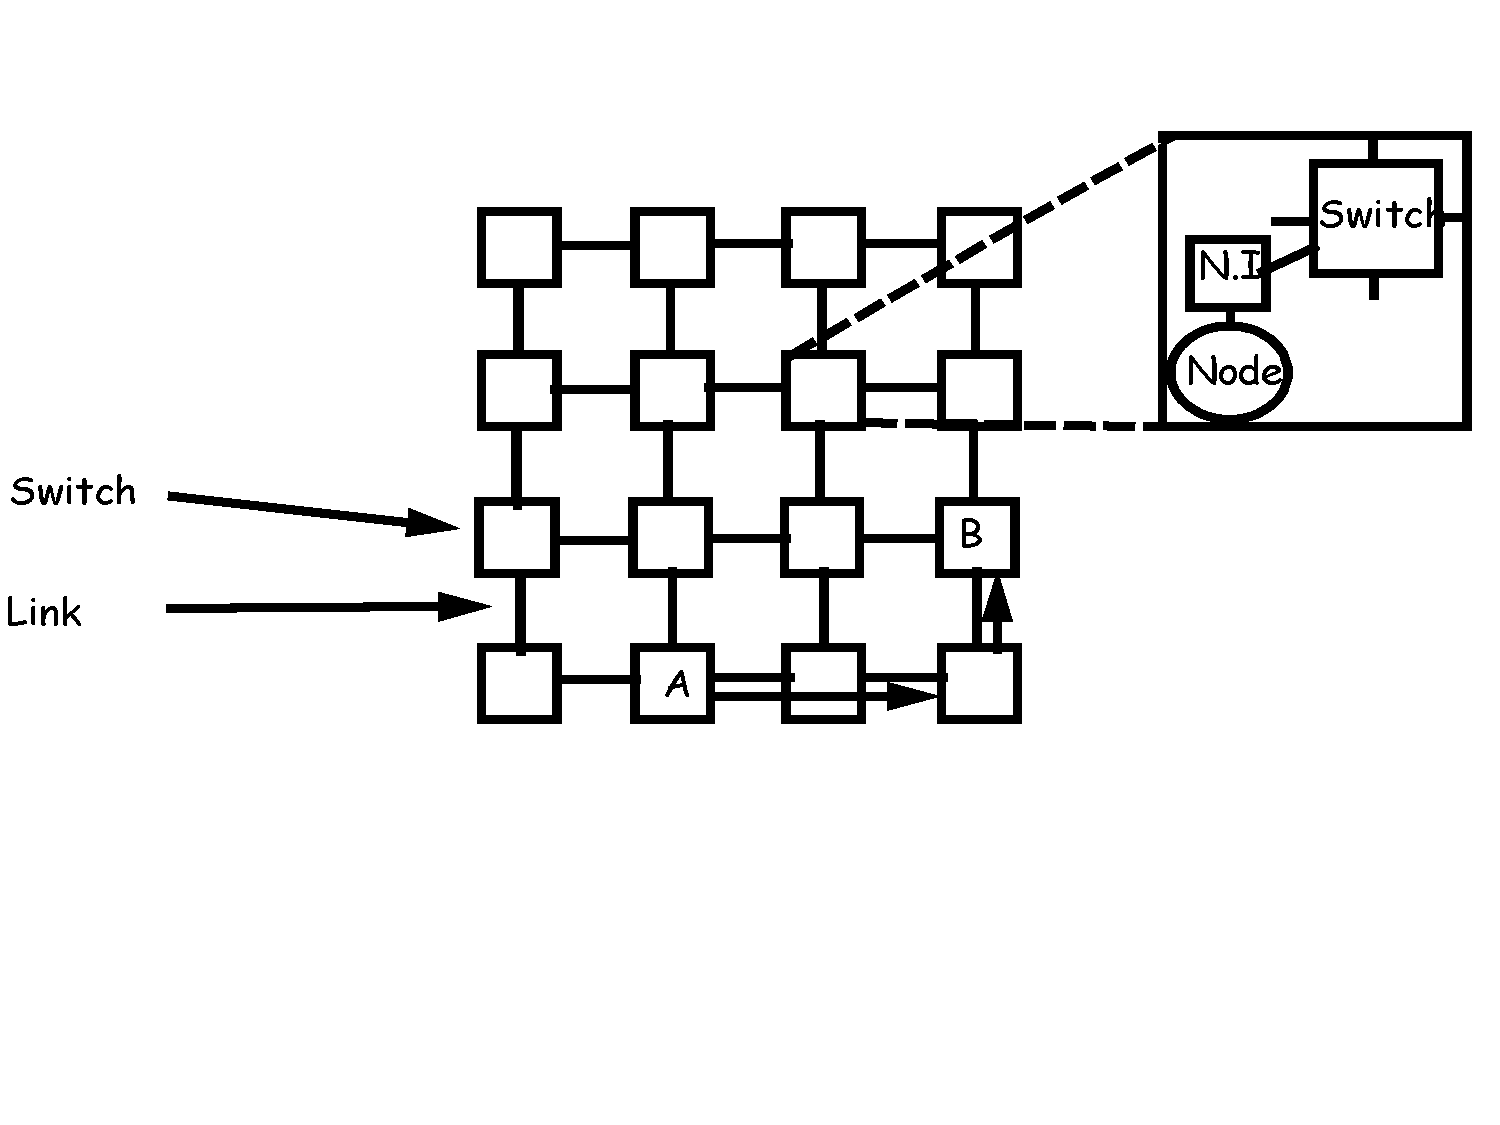
\includegraphics[width=47ex]{FigsInterconnect/Mesh}\pause
\column{0.35\textwidth}
\vspace{-6ex}
\begin{scriptsize}
\begin{itemize}
    \item[NI] (network interface) connects switches to nodes.
    \item[Switch] connects input to output ports.
    \item[Links] wires transferring signals between switches.
    \item[Direct] IN (decentralized): to go from {\tt A} to {\tt B} hop from switch to switch.
\end  {itemize}
\end{scriptsize}
\end{columns}
\vspace{-7ex}

\begin{itemize}
    \item[Link] \emp{width ({\tt w})}: \# bits transf. in 1 clock cycle ({\tt t}).
                \emp{Bandwidth={\tt w/t}}.\\
                \emp{Synch} (use same clock) vs \emp{Asynch} (use handshake) \emp{communic}.\medskip
    \item[Switch] n-by-n switch (input/output ports) $\Rightarrow$ contention to output port
                    $\Rightarrow$ buffering at input or/and output port.
                  Input/output ports (and buffers) often connected by a crossbar switch (later).
\end  {itemize}


\end{frame}


\begin{frame}[fragile,t]
\frametitle{Communication Models}

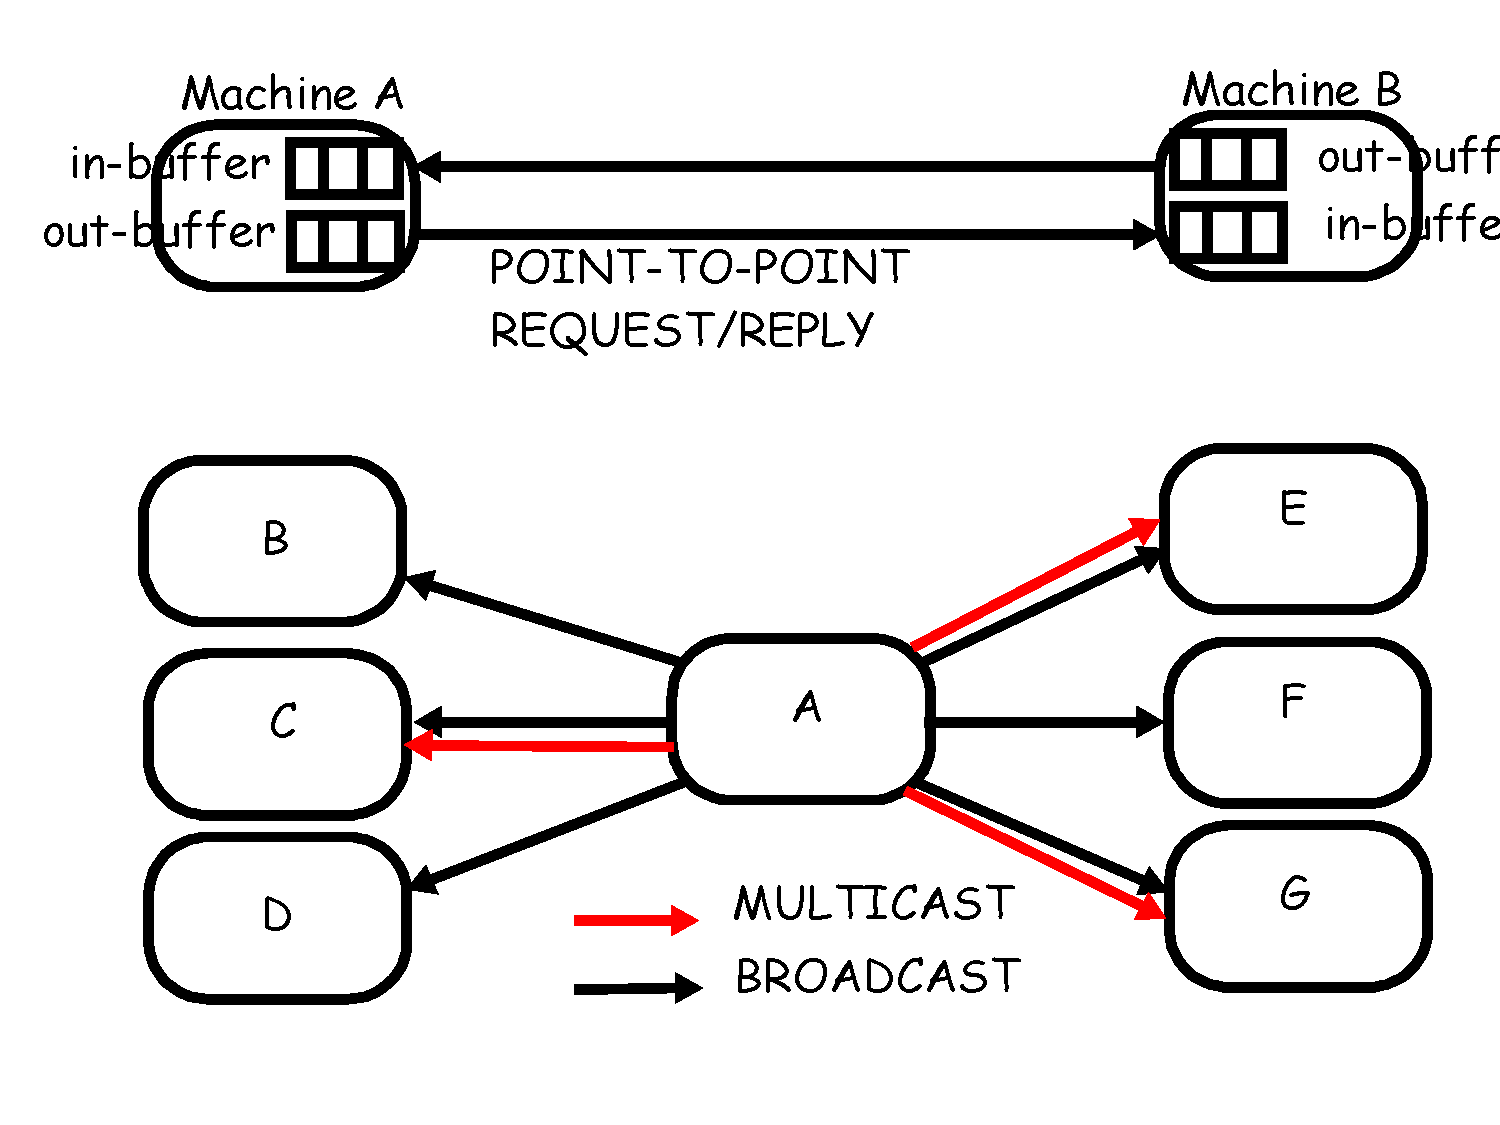
\includegraphics[width=47ex]{FigsInterconnect/SimpleCommun}\pause

\vspace{-2ex}
\begin{itemize}
    \item \emp{point-to-point} message transfer
    \item \emp{request-reply}: request carries ID of sender
    \item \emp{multicast}: one to many
    \item \emp{broadcast}: one to all. 
\end  {itemize}

\end{frame}


\begin{frame}[fragile,t]
\frametitle{Messages and Packets}

%If messages were of arbitrary size they could exhaust resources along a route and delay other transfers.

Messages contain the transferred information. 
\medskip

Messages broken into fixed-size packets, which are sent one by one:
 \center{ 
\includegraphics[width=47ex]{FigsInterconnect/Packet}}\pause

\begin{itemize}
    \item \emp{Payload}: message data, not relevant to interconnect
    \item \emp{Error Code (ECC)}: error/detection correction info because packets 
            can be lost or or corrupted, e.g., radiations or switch/link failures.
    \item \emp{Header/trailer}: routing info + request/response type.
    \item \emp{Packet Envelope}: Header + ECC + Trailer. 
\end  {itemize}

\end{frame}

\begin{frame}[fragile,t]
\frametitle{Eg Bus: indirect, low cost, shared, low bandwidth}

\vspace{-4ex}

\center{ 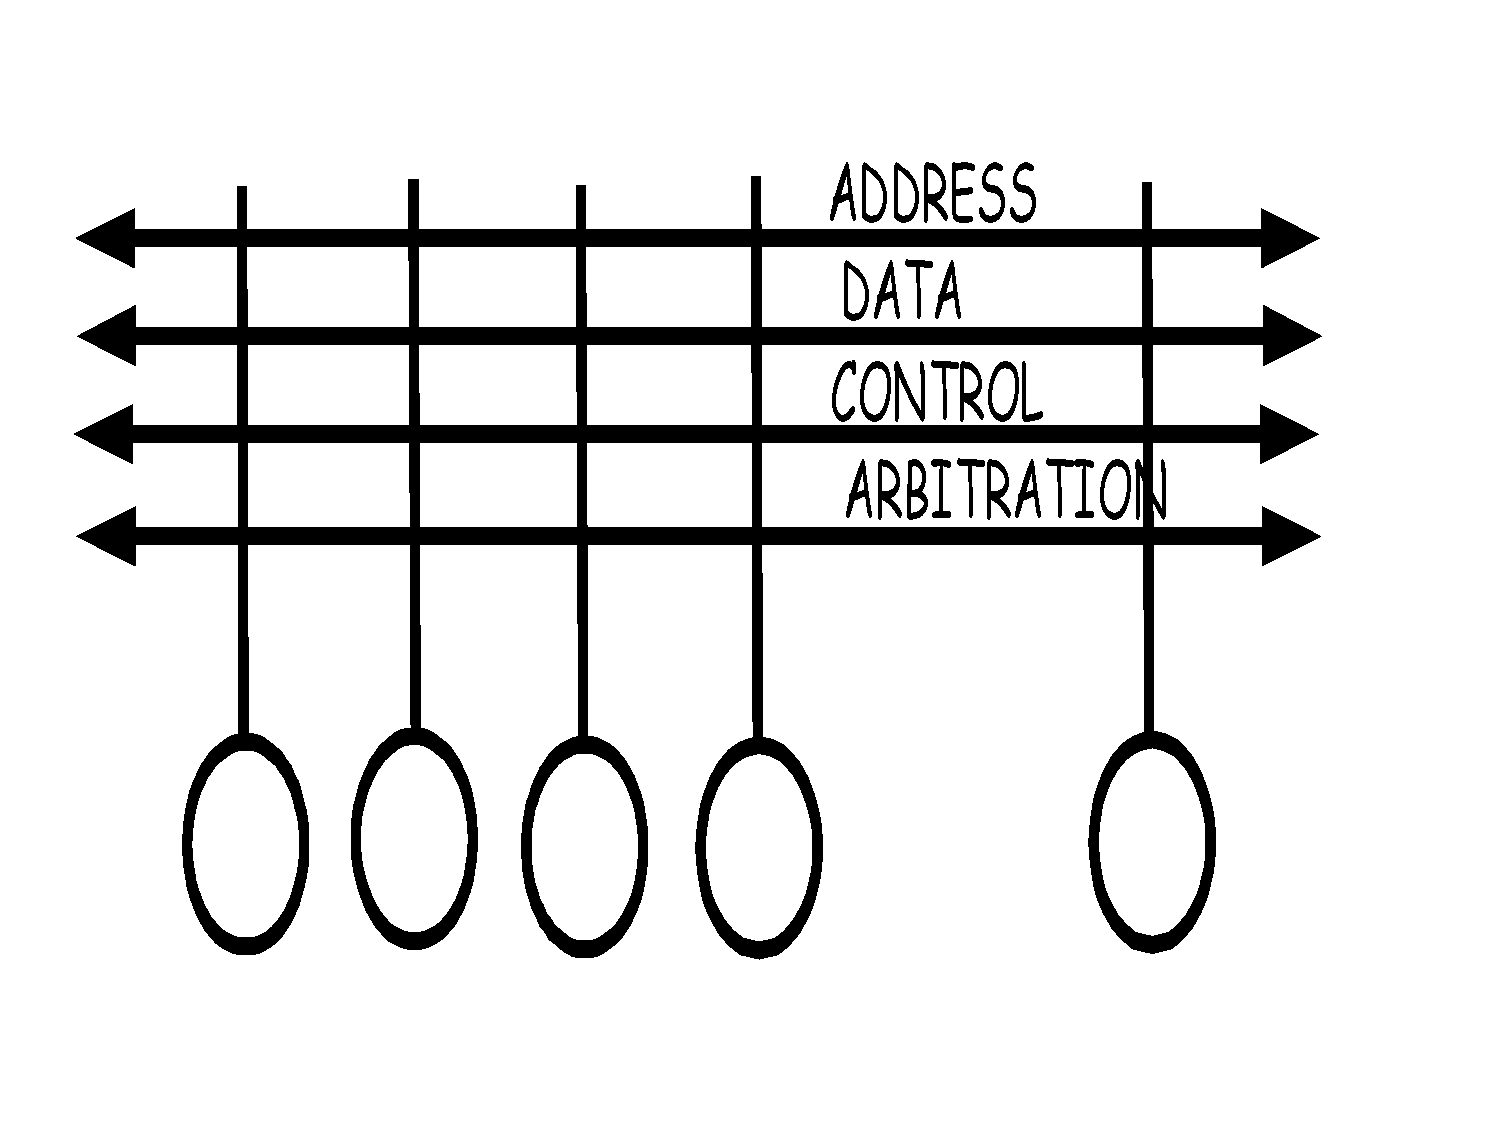
\includegraphics[width=44ex]{FigsInterconnect/Bus}}\pause
\vspace{-4ex}
\begin{itemize}
    \item \emp{Indirect} ({\scriptsize centralized}): box with ports to all nodes exchanging info.
    \item \emp{Shared} medium requires arbitration to grant {\em exclusive access},
    \item \emp{Broadcast/Broadcall} communication,
    \item \emp{Line Multiplexing}, e.g., address, data.
    \item \emp{Pipelining}, e.g., {\tt arbitration $\Rightarrow$ address $\Rightarrow$ data}
    \item \emp{Split transaction} vs \emp{Atomic} (circuit-switched) Bus\bigskip
\end  {itemize}

\end{frame}

\subsection{Switching Strategies: Circuit and Packet Switching}
\begin{frame}[fragile]
	\tableofcontents[currentsubsection]
\end{frame}


\begin{frame}[fragile,t]
\frametitle{Switching Strategy}

\alert{Defines how connections are established in the network.}

\begin{itemize}
    \item[Circuit] (uninterrupted) \emph{Switching}: establishes a route for 
                    the duration of the network service $\Rightarrow$ avoids routing
                    overhead in each switch $\Rightarrow$\\ 
                    Trades off \emph{lower latency} for 
                    \emp{reduced bandwidth of other procs}.\medskip
        \begin{itemize}
            \item Example Remote Memory Read On Atomic Bus:\\
%                        Connect with remote node \& hold the bus while MM is accessed
%                        release the bus only when data has been returned
            \item Example Circuit Switching in MESH:\\
                        Establish path in network, transmit packets/message, release path.\\
                        \emph{Good when packets are sent continuously between two nodes.} 
        \end  {itemize}\bigskip

    \item[Packet] \emph{Switching}: multiplex several services by sending packets with addresses
                $\Rightarrow$ \emp{larger latency}, \emph{higher bandwidth}.\medskip
        \begin{itemize}
            \item Example: Remote Memory Access On Split-Transaction Bus.
%                        Send request to remote node, then release bus while memory is accesses,
%                        other transactions take place, then remote node send reply packet to sender.
%                        release the bus only when data has been returned
            \item Example: Remote memory access on a MESH. 
        \end  {itemize}
\end  {itemize}

\end{frame}


\begin{frame}[fragile,t]
\frametitle{Switching Strategy}

\emph{Two main Packet Switching Strategies:}
\begin{itemize}
    \item[1] \emp{Store-and-Forward:} packets are stored in buffers at each node,
            and cannot leave a node until the whole packet has arrived.\smallskip

    \item[2] \emp{Cut-Through:} packets can move through nodes in pipelined fashion, 
                i.e., entire package moves through several nodes at once.
\end{itemize}
\medskip

In practice we must deal with conflicts by stalling packets.\\
\emph{Two implementations of Cut-Through Packet Switching}:\smallskip
\begin{itemize}
    \item[1] \emp{Virtual Cut-Through:} 
        \begin{itemize}
            \item {\em Each node has enough buffering for the entire packet}, hence
            \item in case of conflict the entire packet is buffered in a node.
            \item When traffic is congested resembles store-and-forward.
        \end  {itemize}\smallskip

    \item[2] \emp{Wormhole:} Def. {\sc phit}: link's width (\# of bits per cycle) 
        \begin{itemize}
            \item {\sc flit} (FlowControlUnit) consists of several consec
                    {\sc phits} of packet% and must contain the routing info.
            \item {\em Each node has enough buffering for one {\sc flit}}, the basic 
                    transfer unit subject to control flow. Virtual cut through: 
                    {\sc fit} is 1 package.
            \item Saves buffering space (precious).
        \end  {itemize}
\end  {itemize}

\end{frame}


\begin{frame}[fragile,t]
\frametitle{Switch Microarchitecture}

\center{ 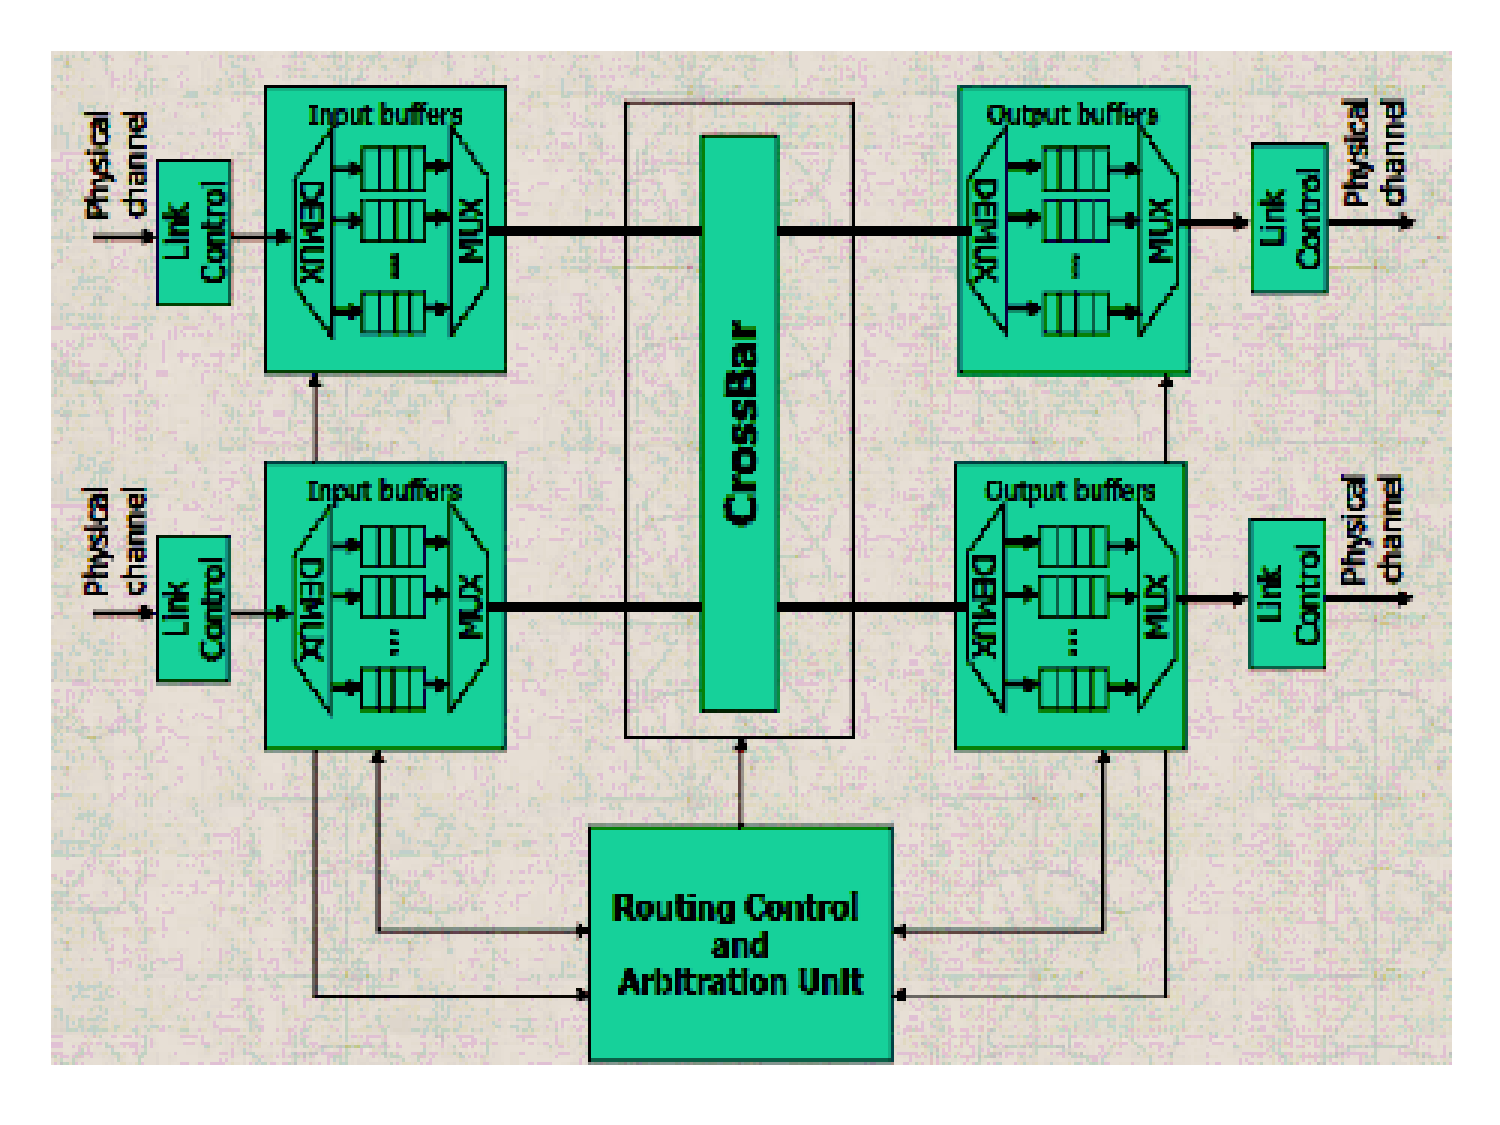
\includegraphics[width=44ex]{FigsInterconnect/SwitchArch}}

{\scriptsize From Duato and Pinkston in Hennessy and Paterson, 4th edition.}
\pause

        \begin{itemize}
            \item Physical Channel $\equiv$ LINK, Virtual Channel $\equiv$ Buffers + LINK
            \item LINK is multiplexed among FLITs
            \item Input Buffering suffers from Head-Of-Line Blocking. 
        \end  {itemize}\smallskip


\end{frame}


\subsection{Latency And Bandwidth Models}
\begin{frame}[fragile]
	\tableofcontents[currentsubsection]
\end{frame}


\begin{frame}[fragile,t]
\frametitle{Latency Models: End-to-End Packet Latency} 

\begin{columns}
\column{0.55\textwidth}
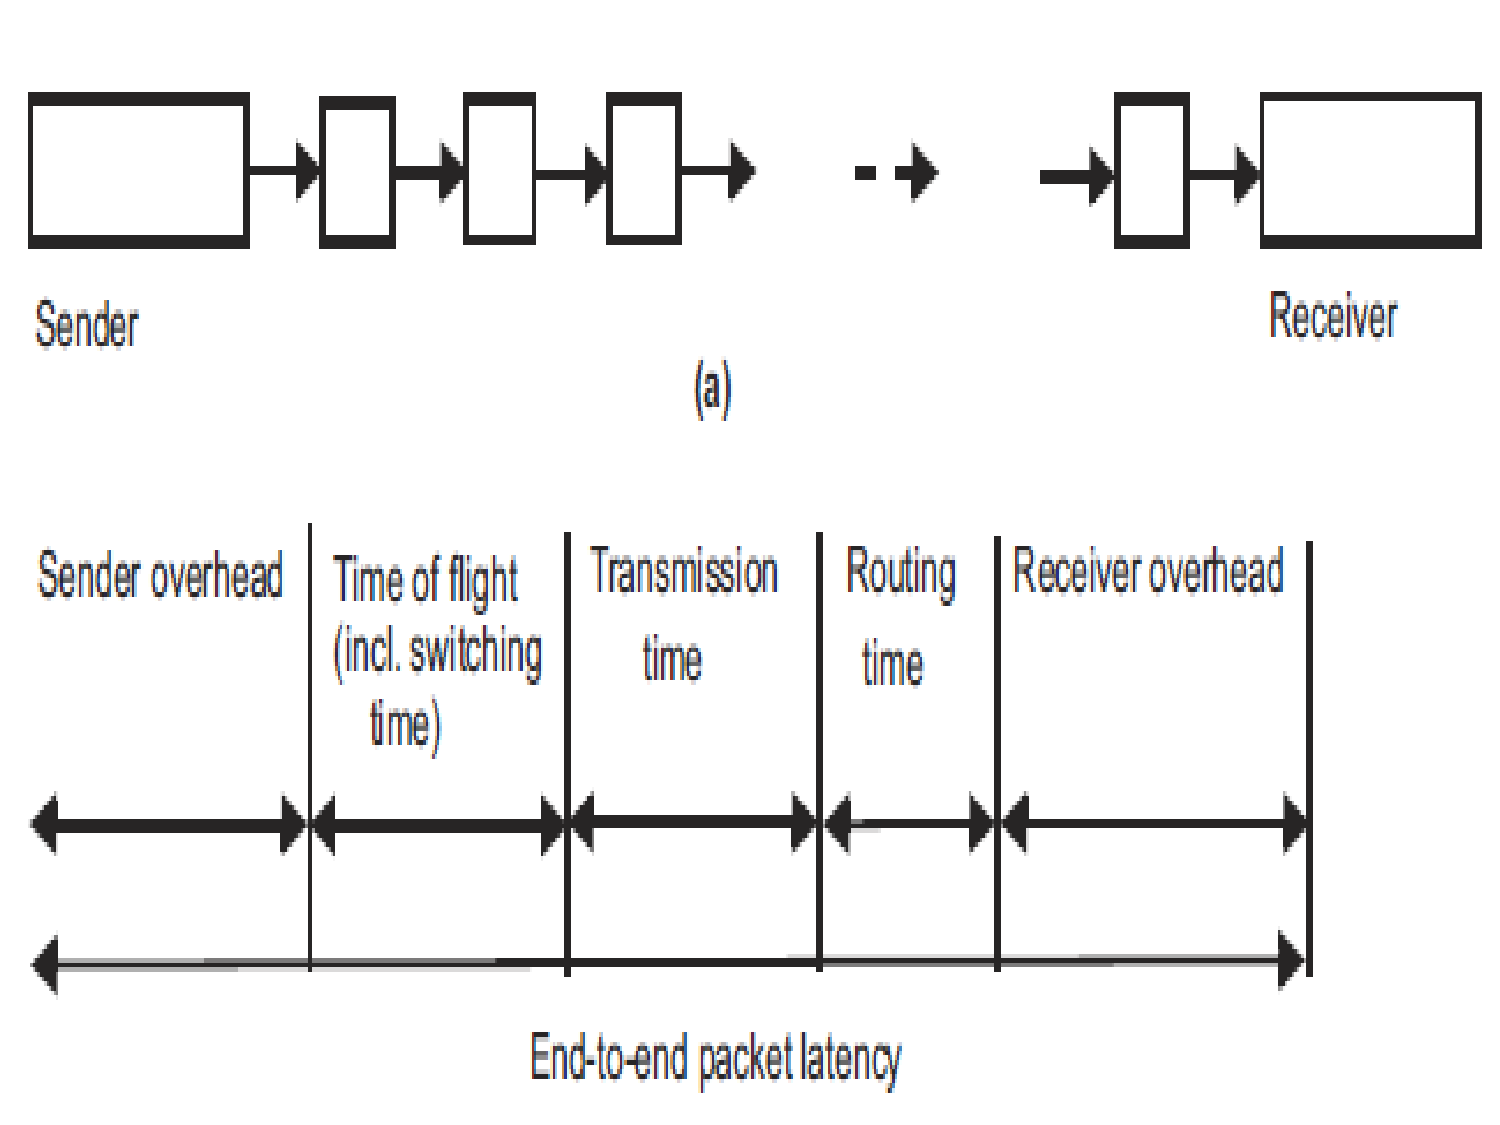
\includegraphics[width=42ex]{FigsInterconnect/LatencyModel}
\column{0.45\textwidth}
\begin{scriptsize}
\begin{itemize}
    \item \emp{SenderOV}erhead: creating the envelope \& moving packet to NI.
    \item \emp{TimeOfFlight}: time to send a bit from source to dest, when
                route is established and without conflicts (includes \emp{SwitchingTime}).
    \item \emp{TransmissionTime}: time to transfer a packet from source to dest, once
                the first bit has arrived @dest,e.g.,{\tt PacketSize/PHITsize}.
    \item \emp{RoutingTime}: time to set up switches (globally/locally).
    \item \emp{SwitchingTime}: depends on switching strategy.
    \item \emp{ReceiverOV}erhead: time to strip envelope and move packet in.
%    \item {\sc phit}: number of bits transferred on a link per cycle
%    \item {\sc flit}: control flow unit (several consecutive {\sc phit}s of a packet).
\end  {itemize}
\end{scriptsize}
\end{columns}
\bigskip

\alert{\tt End-to-End Packet Latency =} \emp{\tt SenderOV + TimeOfFlight + }
\emp{\tt~~~~~~~~~~~~~~~~~~~~~~~~~~~~TransmissionTime + }
\emp{\tt~~~~~~~~~~~~~~~~~~~~~~~~~~~~RoutingTime + ReceiverOV}

\end{frame}

\begin{frame}[fragile,t]
\frametitle{Latency Models (Continuation)}

\emph{Measures of Latency:}
\begin{itemize}
    \item \emp{Routing Distance}: \# of links traversed by a packet
    \item \emp{Average Routing Distance}: average over all node pairs.
    \item \emp{Network Diameter}: longest routing distance over all node pairs.
\end  {itemize}\medskip

\emph{Packets of a Message Can Be Pipelined:}
\begin{itemize}
    \item Transfer pipeline has three stages: {\tt SendrOV$\rightarrow$Transmission$\rightarrow$ReceiverOV}
    \item {\tt TotalMsgTime = Time for First Packet +}\\ 
          {\tt~~~~~~~~~~~~~~~~(N-1) / Pipeline Throughput} 
\end  {itemize}\medskip

\alert{\tt End-to-End Msg Latency=}\emp{\tt SenderOV + TimeOfFlight + }\\
\emp{\tt~~~~~~~~~~~~~~~~~~~~~~~TransmissionTime + RoutingTime +}\\
\emp{\tt~~~~~~~~~~~~~~~~~~~~~~~(N-1) $\times$ Max(SenderOV,}\\
\emp{\tt~~~~~~~~~~~~~~~~~~~~~~~~~~~~~~~~~~~~TransmissionTime,}\\
\emp{\tt~~~~~~~~~~~~~~~~~~~~~~~~~~~~~~~~~~~~ReceiverOV)}

\end{frame}


\begin{frame}[fragile,t]
\frametitle{Latency for Switching Strategies}

\emph{Circuit Switching:}
\begin{itemize}
    \item Route is set up first, \emp{\tt RoutingTime = L$\times$R + TimeOfFlight}
    \item {\tt R}: to set each switch, {\tt L}: \# of switches,\\
          {\tt TimeOfFlight}: because I need to inform the node back.
\end  {itemize}\medskip

\emph{Packets Switching:} rout set up as package moves through switches

\center{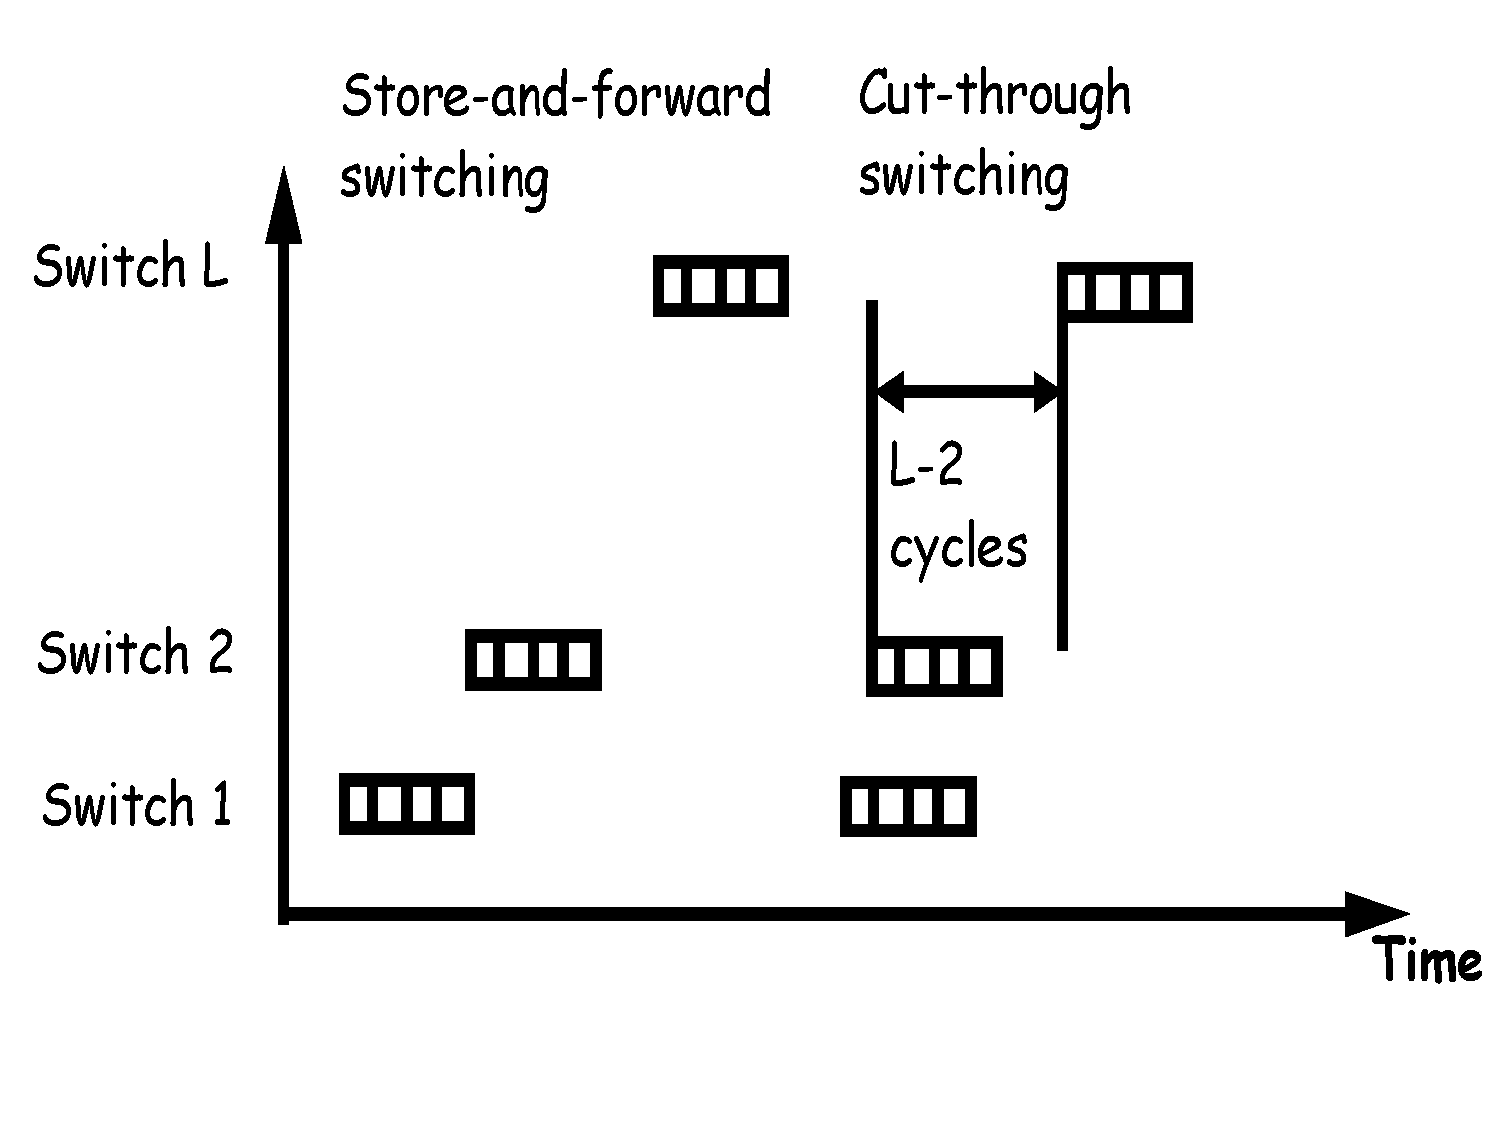
\includegraphics[width=44ex]{FigsInterconnect/SwitchingStartegies}}

\end{frame}

\begin{frame}[fragile,t]
\frametitle{Latency for Switching Strategies (Cont.)}

\alert{\scriptsize {\tt PacketLatency = SenderOV + ToF (incl. SwitchingTime) + TransmissionTime +}}\\
\alert{\scriptsize {\tt~~~~~~~~~~~~~~~~RoutingTime + ReceiverOV}}
\medskip

{\scriptsize {\tt R}: routing time per switch, {\tt N}: \# of phits, 
             {\tt L}: \# of switches, {\tt ToF}: time of flight}

\begin{itemize}
    \item \emph{Packet Latency for Circuit Switching}
        \begin{itemize}
            \item \emp{\tt SenderOV + 2$\times$ToF + N + L$\times$R + ReceiverOV}
            \item \emp{\tt ToF = L} because there are {\tt L} switches and {\tt 1} {\sc phit} to switch.
        \end  {itemize}

    \item \emph{Packet Latency for Store and Forward}
        \begin{itemize}
            \item \emp{\tt SenderOV + ToF + N + L$\times$R + ReceiverOV}
            \item \emp{\tt ToF = L$\times$N} because switching involves the whole packet in {\sc phit}s.
        \end  {itemize}

    \item \emph{Packet Latency for Cut Through}
        \begin{itemize}
            \item \emp{\tt SenderOV + ToF + N + L$\times$R + ReceiverOV}
            \item \emp{\tt ToF = L} as in circuit switching when traffic \emph{not congested}.
            \item \emp{\tt ToF = L$\times$N} as in store and forward when \alert{traffic congested}.
        \end  {itemize}

    \item \emph{Virtual Cut Through \& Wormhole Cut Switching} similar to circuit switching
            when traffic not congested, but offers \emph{better bandwidth}.
            Differences reside in how they handle conflicts. 
\end  {itemize}
\end{frame}

\begin{frame}[fragile,t]
\frametitle{Bandwidth Models}

\begin{itemize}
    \item Bottlenecks Increase Latency, but Transfers are Pipelined:\\
          \emp{\tt Effective Bandwidth = PacketSize / }\\
                    \emp{\tt~~~~~~~~~~~~~~MAX(SenderOV,ReceiverOV,TransmissionTime)}\medskip

    \item Network contention affects latency and effective bandwidth\\
            (not acounted in above formula).\medskip

    \item \emp{Bisection Width:}
        \begin{itemize}
            \item network seen as a graph: vertices are switches and edges are links,
            \item Bisection is a cut through a minimum set of edges such that
                    the cut divides the network graph into two isomorphic subgraphs.
            \item \emp{Measures bandwidth when all nodes in one subgraph communicate 
                        only with nodes in the other subgraph.}
        \end  {itemize}\medskip

    \item \emp{Aggregate Bandwidth}: is the bandwidth across all links divided by
                the number of nodes. 
\end  {itemize}
\end{frame}

\subsection{Indirect Interconnect-Network Topologies}
\begin{frame}[fragile]
	\tableofcontents[currentsubsection]
\end{frame}

\begin{frame}[fragile,t]
\frametitle{Crossbar Switch \& Multistage IN (MIN)}

Indirect Networks: centralized, typically connect different types of nodes, 
e.g., private with shared caches, cores to shared caches/mem.

\vspace{-1ex}
\center{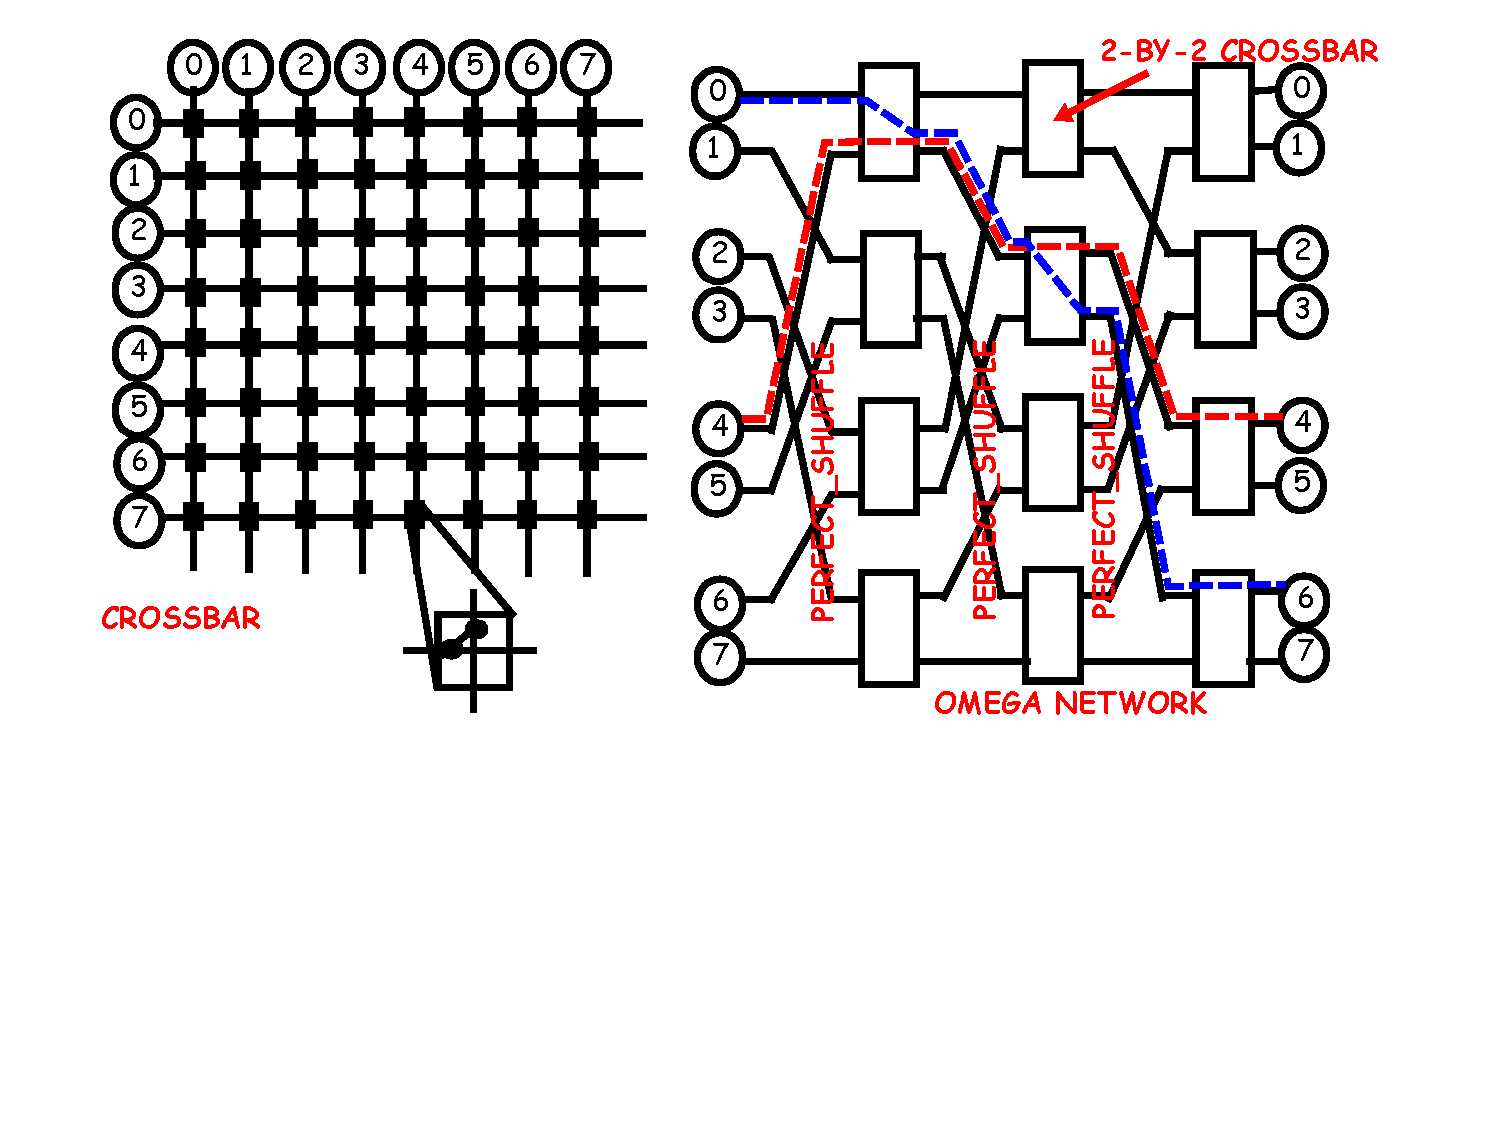
\includegraphics[width=55ex]{FigsInterconnect/CrossbarAndMultiStage}}\pause
\vspace{-15ex}

\begin{scriptsize}
\begin{columns}
\column{0.50\textwidth}
\emp{N$\times$N Crossbar:} N vertical \& N horizontal buses. Routing Mechanism
controls all \emp{N$^2$ crosspoints}, each of them may connect two buses $\Rightarrow$
unicast, multicast, and broadcast.\\
\emph{Bandwidth scales linearly with N}, but 
\alert{limited by bus length/load and cost/resource.}

\column{0.59\textwidth}
Use k$\times$k crossbars as building blocks.\\
\emp{Perfect shuffle exchange} (deck of cards)!\\
{\tt N$\times$N} nodes requires \emph{\tt (N$\times$log$_k$N)/k} crossbars,\\
but a packet passes through \emp{\tt log$_k$N} crossbars!\\
MIN's \emph{cost scales better}, but \alert{prone to contention}.
\end{columns}
\end{scriptsize}
\end{frame}

\begin{frame}[fragile,t]
\frametitle{Tree \& Butterfly IN}

Topology impacts the routes that share resources \& cause conflicts.

\medskip

\begin{columns}
\column{0.63\textwidth}
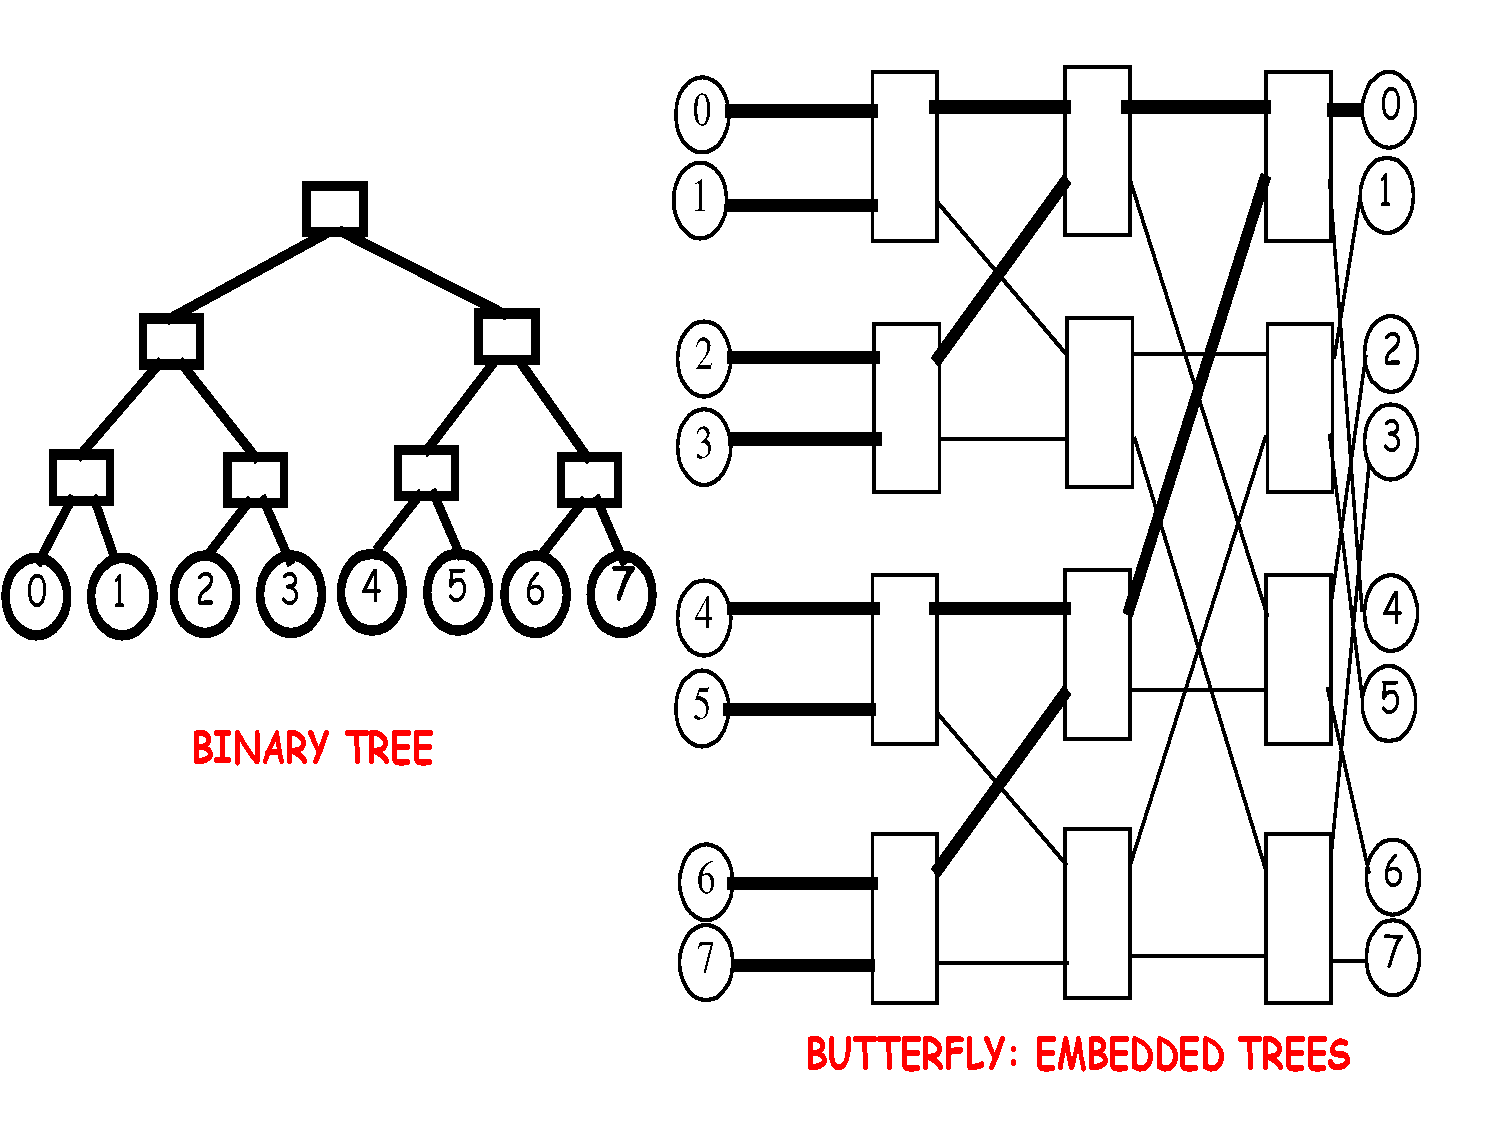
\includegraphics[width=48ex]{FigsInterconnect/BTreeButerfly}
\column{0.44\textwidth}
\begin{scriptsize}
\begin{itemize}
    \item \alert{In the butterfly network: are there any trees that do not share resources?}\pause
    \item \emp{k-ary Tree} connecting N nodes has depth {\tt log$_k$N} \& exploits locality
                 but \alert{bisection width is 1.}\\
    \item \emp{Fat tree}: the closer the link to root, the higher its bandwidth. 
    \item \emp{Butterfly Networks}: is a MIN in which trees are embedded.\\
            There are as many tree roots as \# of nodes N, but different trees
            may share resources.
\end  {itemize}
\end{scriptsize}
\end{columns}

\end{frame}


\subsection{Direct Interconnect-Network Topologies}
\begin{frame}[fragile]
	\tableofcontents[currentsubsection]
\end{frame}

\begin{frame}[fragile,t]
\frametitle{Linear Array, Ring, Mesh and Tori}

\emp{Direct (Decentralized) IN}: nodes, typically of same type, are directly 
connected \& integrated tightly with switches $\Rightarrow$ \emph{exploit locality}.

\medskip
\alert{What is the diameter \& bisection of a N=64-nodes Tori?}

\begin{columns}
\column{0.63\textwidth}
\vspace{-2ex}
\center{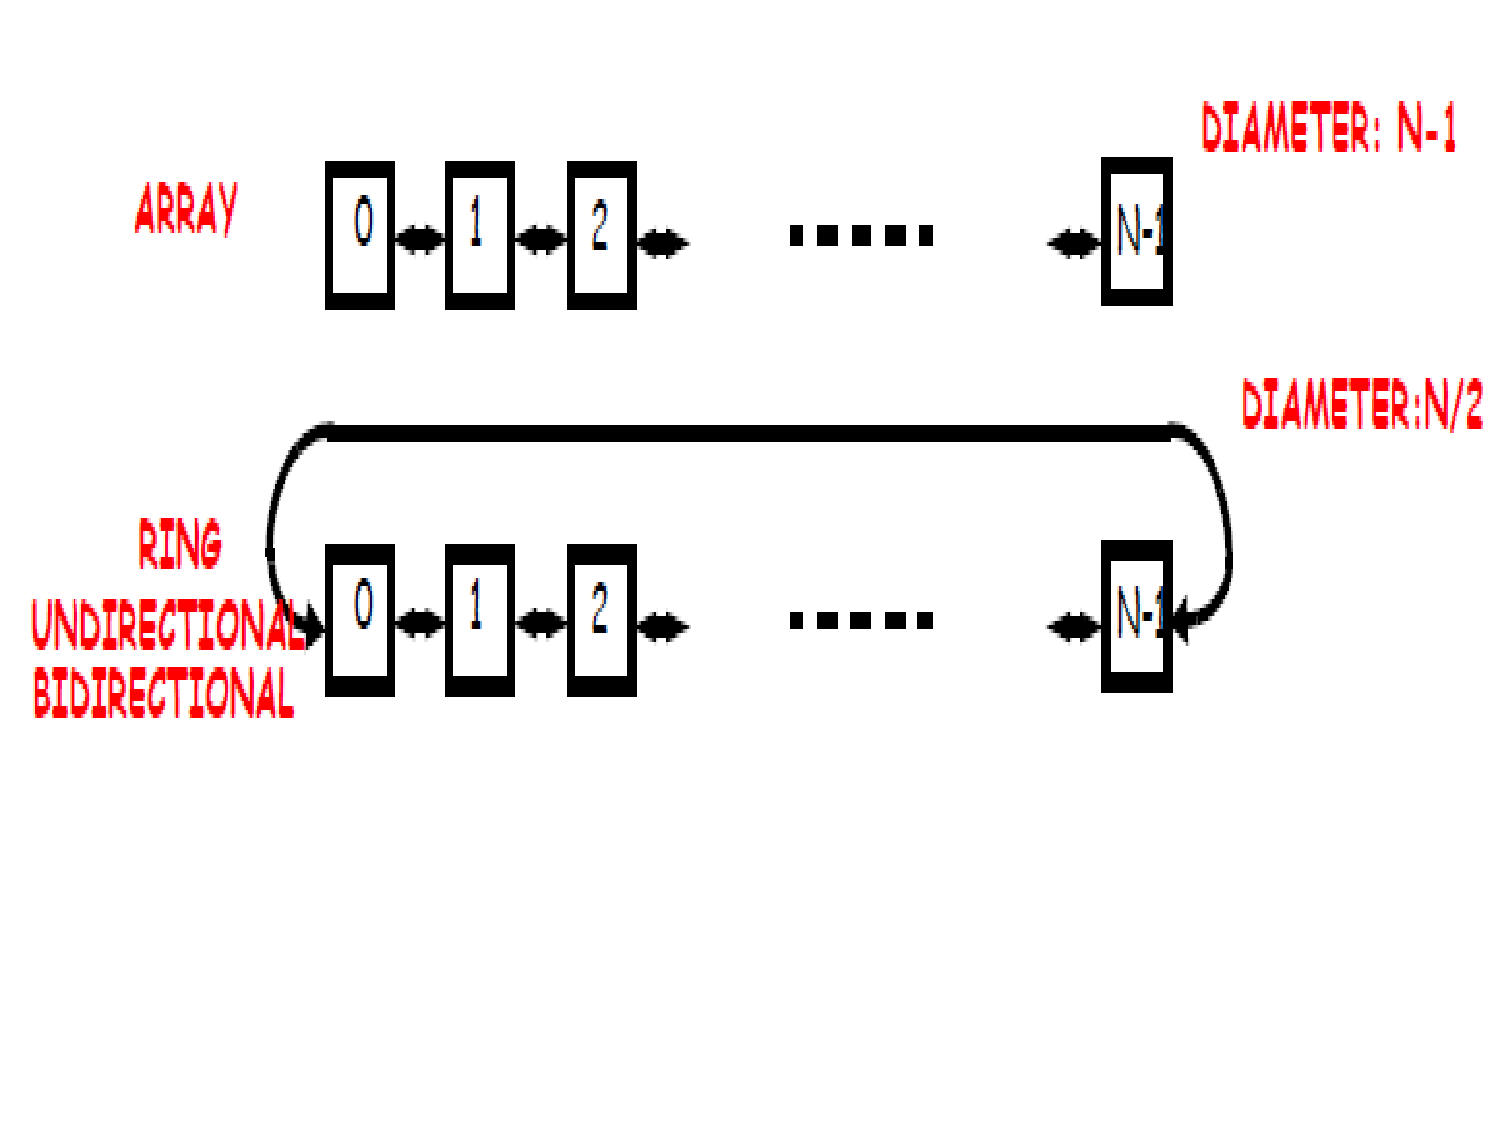
\includegraphics[width=37ex]{FigsInterconnect/ArrayRing}}
\vspace{-11ex}

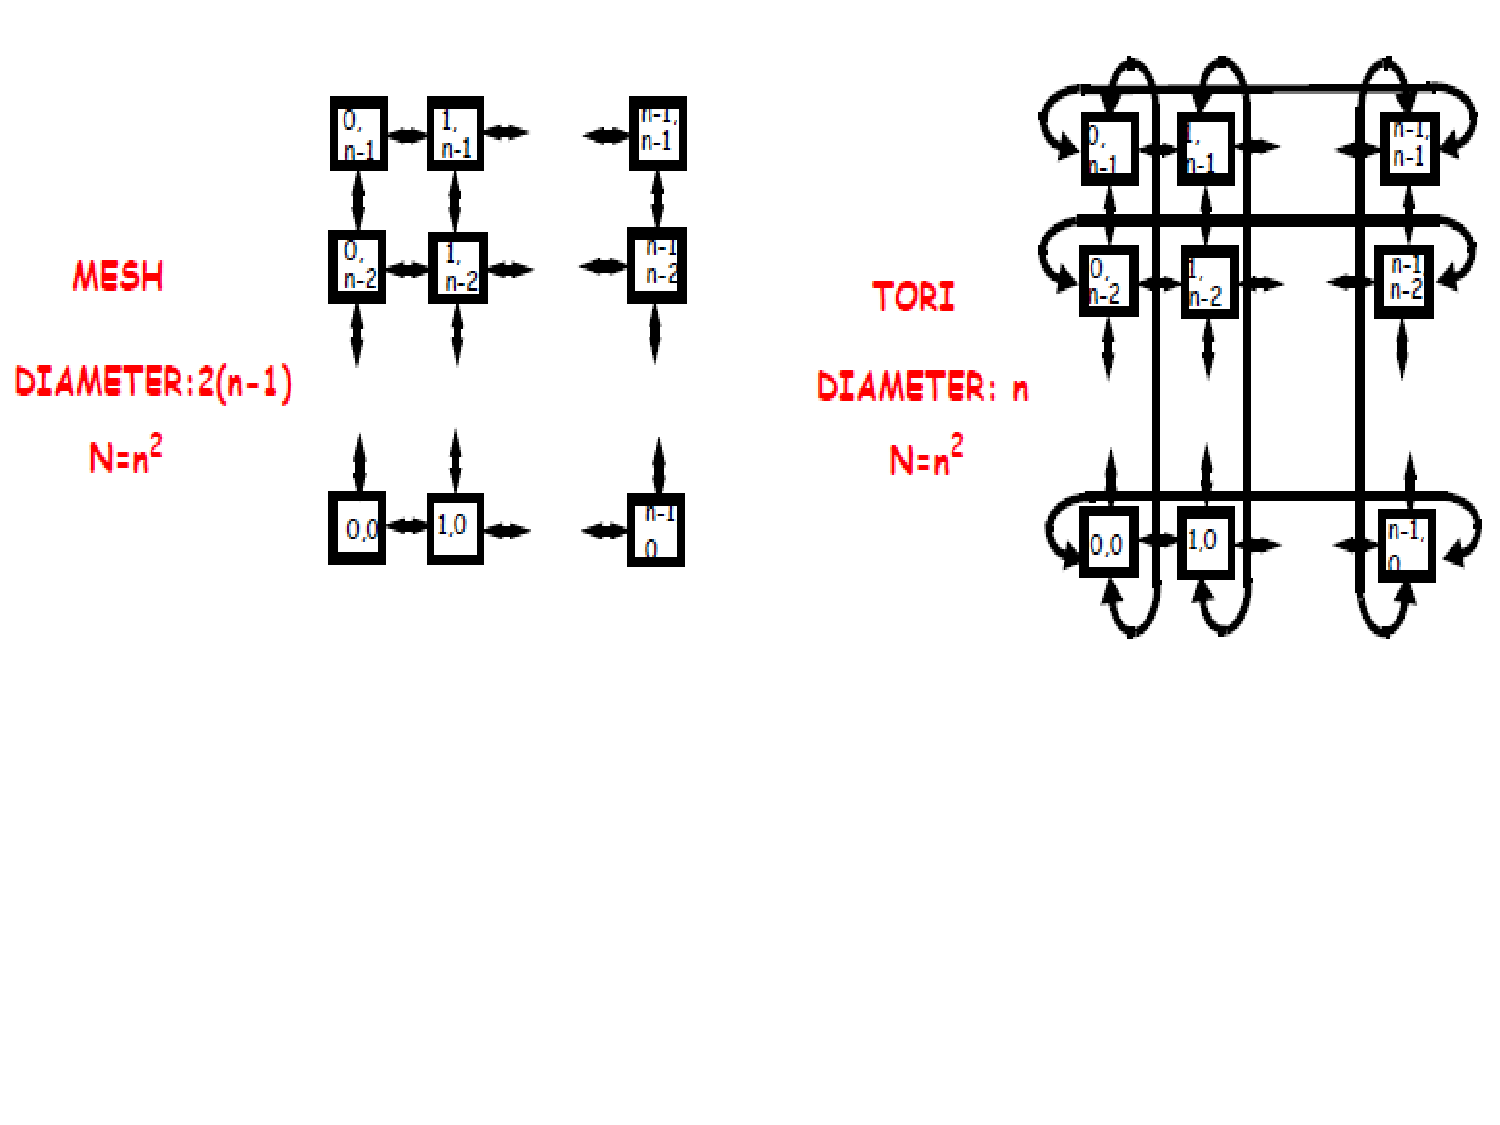
\includegraphics[width=44ex]{FigsInterconnect/MeshTori}\pause
\column{0.33\textwidth}
\vspace{-10ex}
%\begin{scriptsize}
\begin{itemize}
    \item[Array] diameter: {\tt N-1},\\ bisection: {\tt 1}\medskip
    \item[Ring]  diameter: {\tt N/2},\\ bisection: {\tt 2}.\bigskip
    \item[Mesh]  diameter: {\tt 2$\times$n-2}\\ bisection: {\tt n},\\ where {\tt N = n$^2$}.\medskip 
    \item[Tori]  diameter: {\tt n-1},\\ bisection: {\tt 2$\times$n},\\ where {\tt N = n$^2$}.\medskip
\end  {itemize}
%\end{scriptsize}
\end{columns}

\end{frame}


\begin{frame}[fragile,t]
\frametitle{Hypercubes and k-ary n-cubes}

\emp{Direct (Decentralized) IN}: nodes, typically of same type, are directly 
connected \& integrated tightly with switches $\Rightarrow$ \emph{exploit locality}.

\begin{columns}
\column{0.63\textwidth}
\center{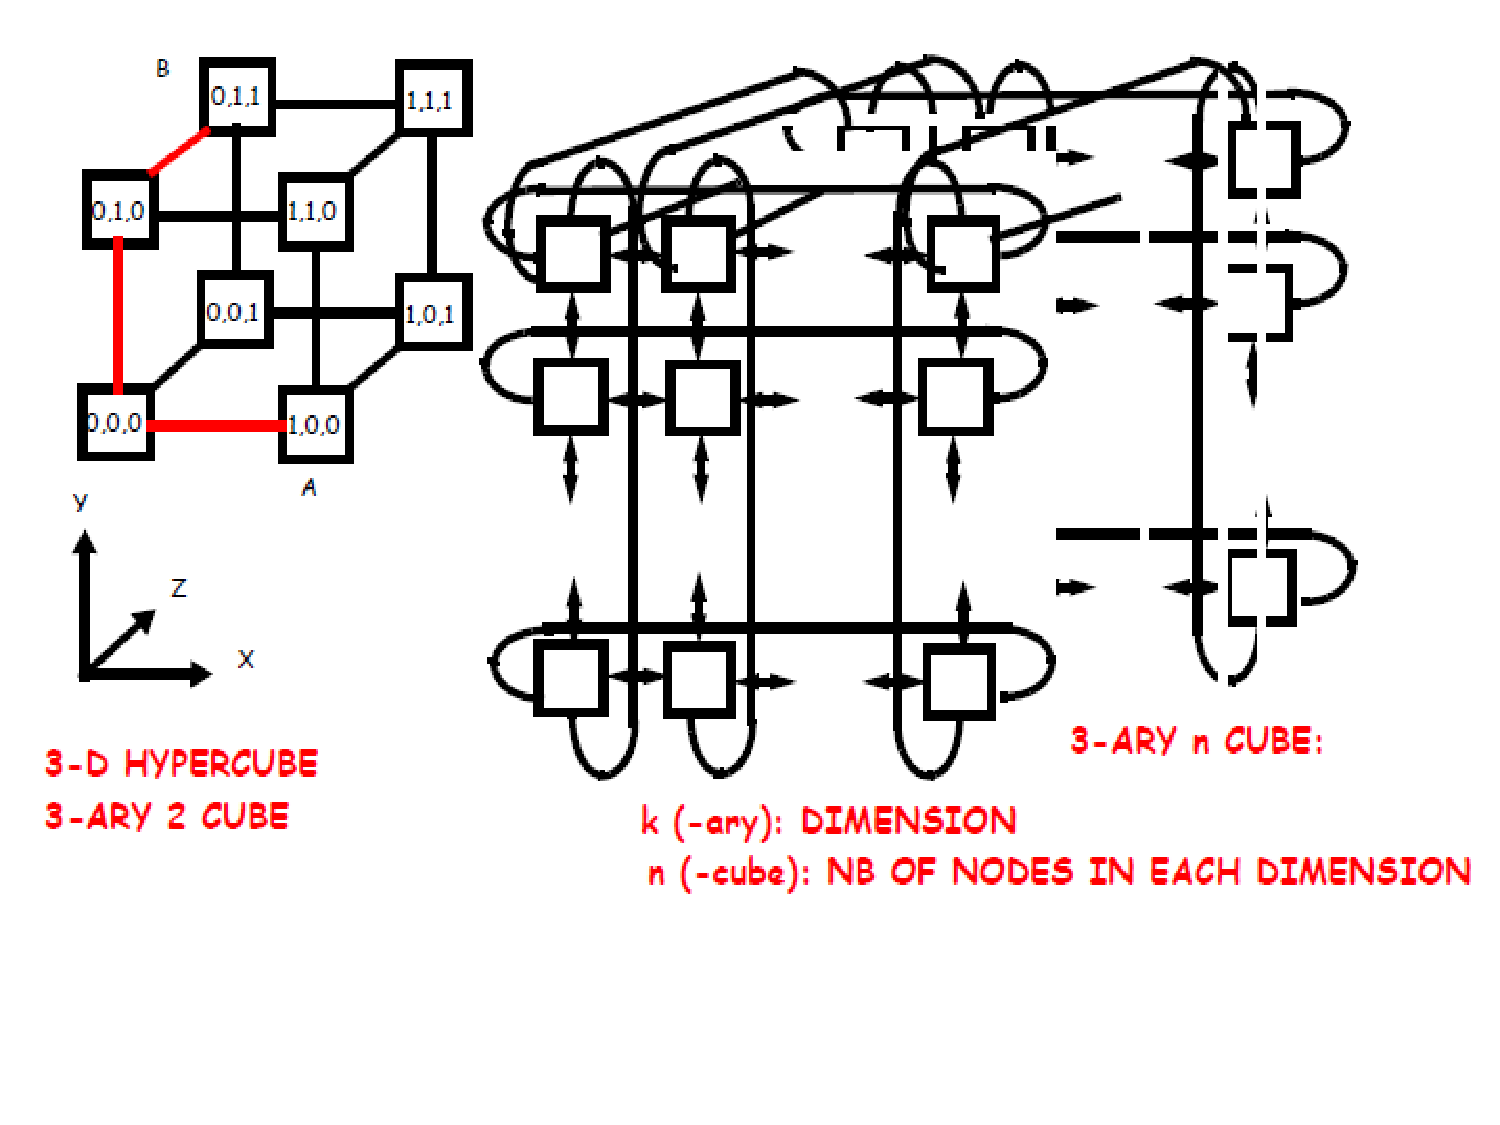
\includegraphics[width=49ex]{FigsInterconnect/Hypercube}}\pause

\column{0.39\textwidth}
\begin{scriptsize}
\begin{itemize}
    \item \emp{Hypercube}: an $n$-dim cube with 2 nodes in each dim.\\
                           Connects \emph{\tt N=$2^n$} nodes, with
          \emph{diameter: {\tt log N} and bisection: $N/2$}, \alert{but}\\
            \alert{the cost (switch degree) of a node grows linear with {\tt n} and 
            hypercube difficult to lay out such that all links are equal!}\bigskip

    \item \emp{k-ary n-Cube}, e.g., hypercube: n-ary 2-cube, n-by-n Tori: 2-ary n-cube.\\  
           3-ary n-cube: built from n Tori connected on top of each over.\bigskip
    
\end  {itemize}
\end{scriptsize}
\end{columns}

\end{frame}

\begin{frame}[fragile,t]
\frametitle{Comparison Between Topologies}

\begin{tabular}{|c|c|c|c|c|}
\hline
Interconnect    & Switch & Network & Bisection & Network \\
Network         & Degree & Diameter& Width     & Size    \\\hline
Crossbar        & N      & 1       & N         & N       \\
Switch          &        &         &           &         \\\hline
Butterfly from  & k      & log$_k$N& N/2       & N       \\
k-by-k switches &        &         &           &         \\\hline
k-ary Tree      & k+1    &2log$_k$N& 1         & N       \\\hline
Linear Array    & 2      & N-1     & 1         & N       \\\hline
Ring            & 2      & N/2     & 2         & N       \\\hline
n-by-n mesh     & 4      & 2(n-1)  & n         & N=n$^2$ \\\hline
n-by-n tori     & 4      & n       & 2n        & N=n$^2$ \\\hline
k-dim hypercube & k      & k       & $2^{k-1}$ & N=$2^k$ \\\hline
k-ary n-cube    & 2k     & nk/2    & 2n$^{k-1}$  & N=n$^k$  \\\hline\hline
\end{tabular}

\begin{scriptsize}
\begin{itemize}
    \item \emp{Switch Degree:} \# of ports for each switch (switch complexity), \emp{approximates cost}.
    \item \emp{Network Diameter:} worst case routing distance between 2 nodes.
    \item \emp{Bisection Width:} \# of links cut in a bisection (measures potential \emp{bottlenecks}).
    \item \emp{Network Size:} \# of nodes  (We used \# for number of).
\end{itemize}
\end{scriptsize}
\end{frame}

\subsection{Routing Algorithms and Deadlock Avoidance}
\begin{frame}[fragile]
	\tableofcontents[currentsubsection]
\end{frame}

\begin{frame}[fragile,t]
\frametitle{Flow Control}

Refers to mechanisms to handle conflicts in switch-based networks.

\begin{columns}
\column{0.70\textwidth}
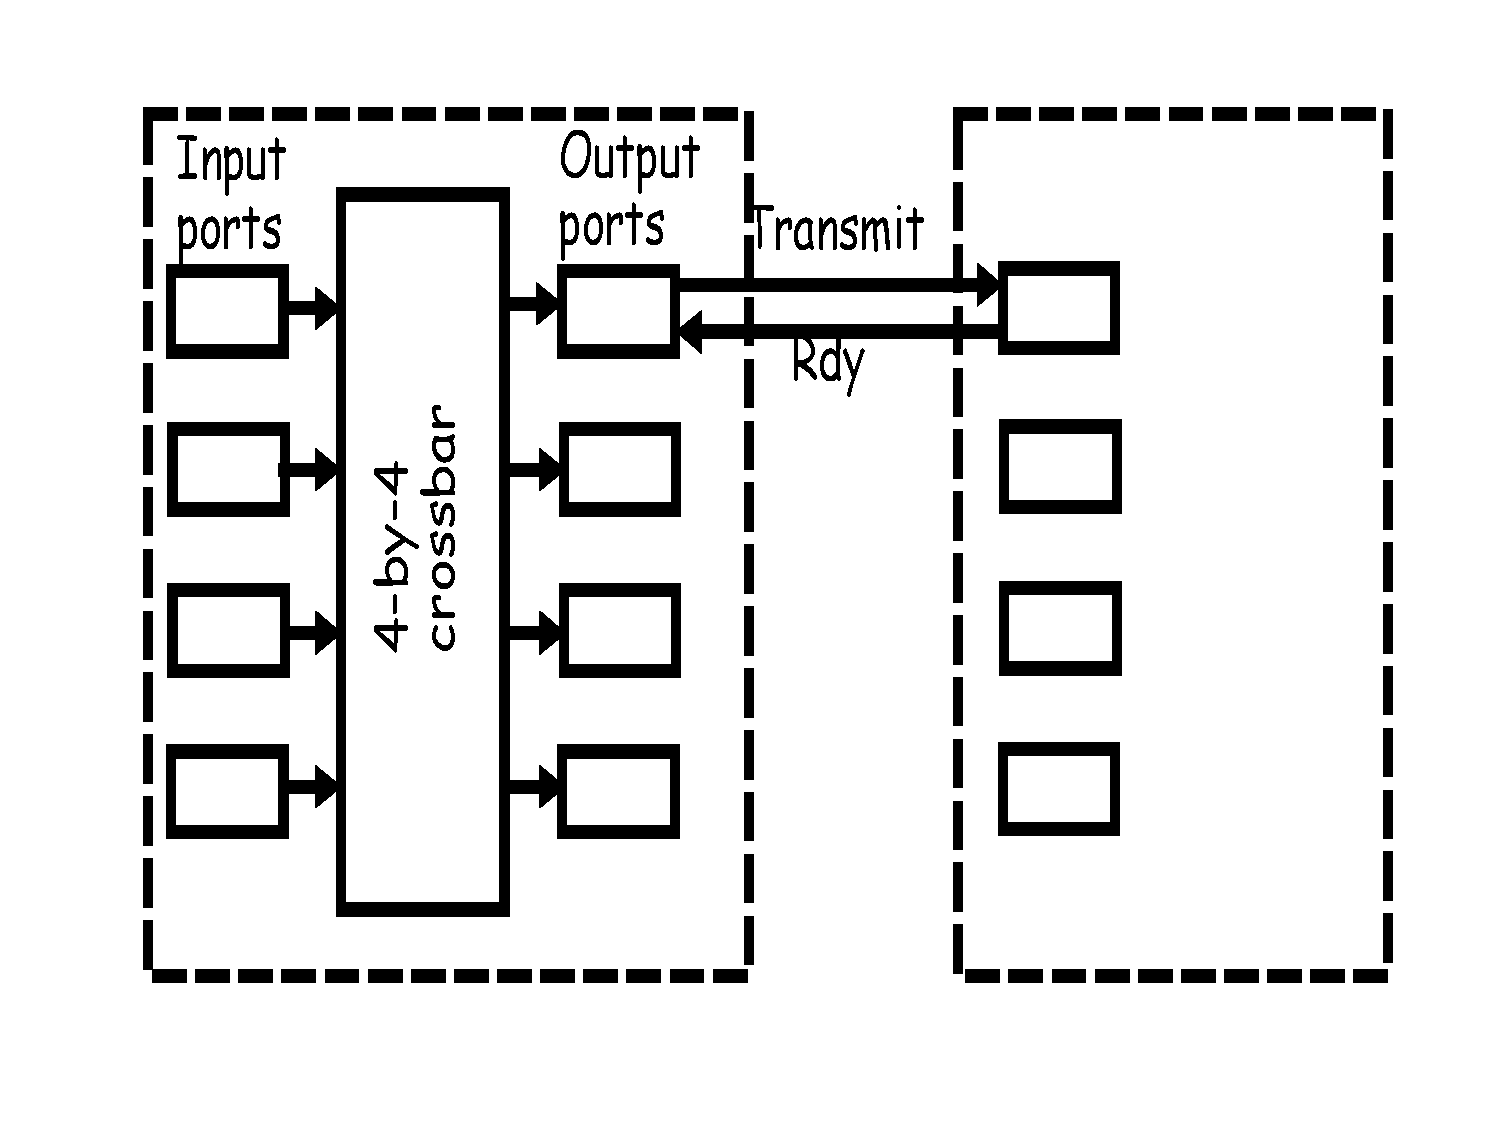
\includegraphics[width=50ex]{FigsInterconnect/Conflicts1}
\column{0.44\textwidth}
\vspace{-1ex}
%\begin{scriptsize}
\begin{itemize}
    \item Buffers at input and output ports.\\
          Virtual Cut Through: buffer for entire packet.\\
          Wormhole: buffer for integral number of {\sc flit}s.\medskip
    \item \emp{Link-Level Flow Control}, e.g., by handshake signal:\\
            {\tt Rdy} indicates whether {\sc flit}s can be transmitted to destination. 
    \item Hot Spot Contention and Tree Saturation. 
\end  {itemize}
%\end{scriptsize}
\end{columns}

\end{frame}

\begin{frame}[fragile,t]
\frametitle{Routing Algorithm for Omega (Shuffle) Network}

\emph{Routing Algorithms}: use source/destination address, \emph{are very simple} $\Rightarrow$ 
keep latency small. (Table driven approaches are prohibitive.)

\center{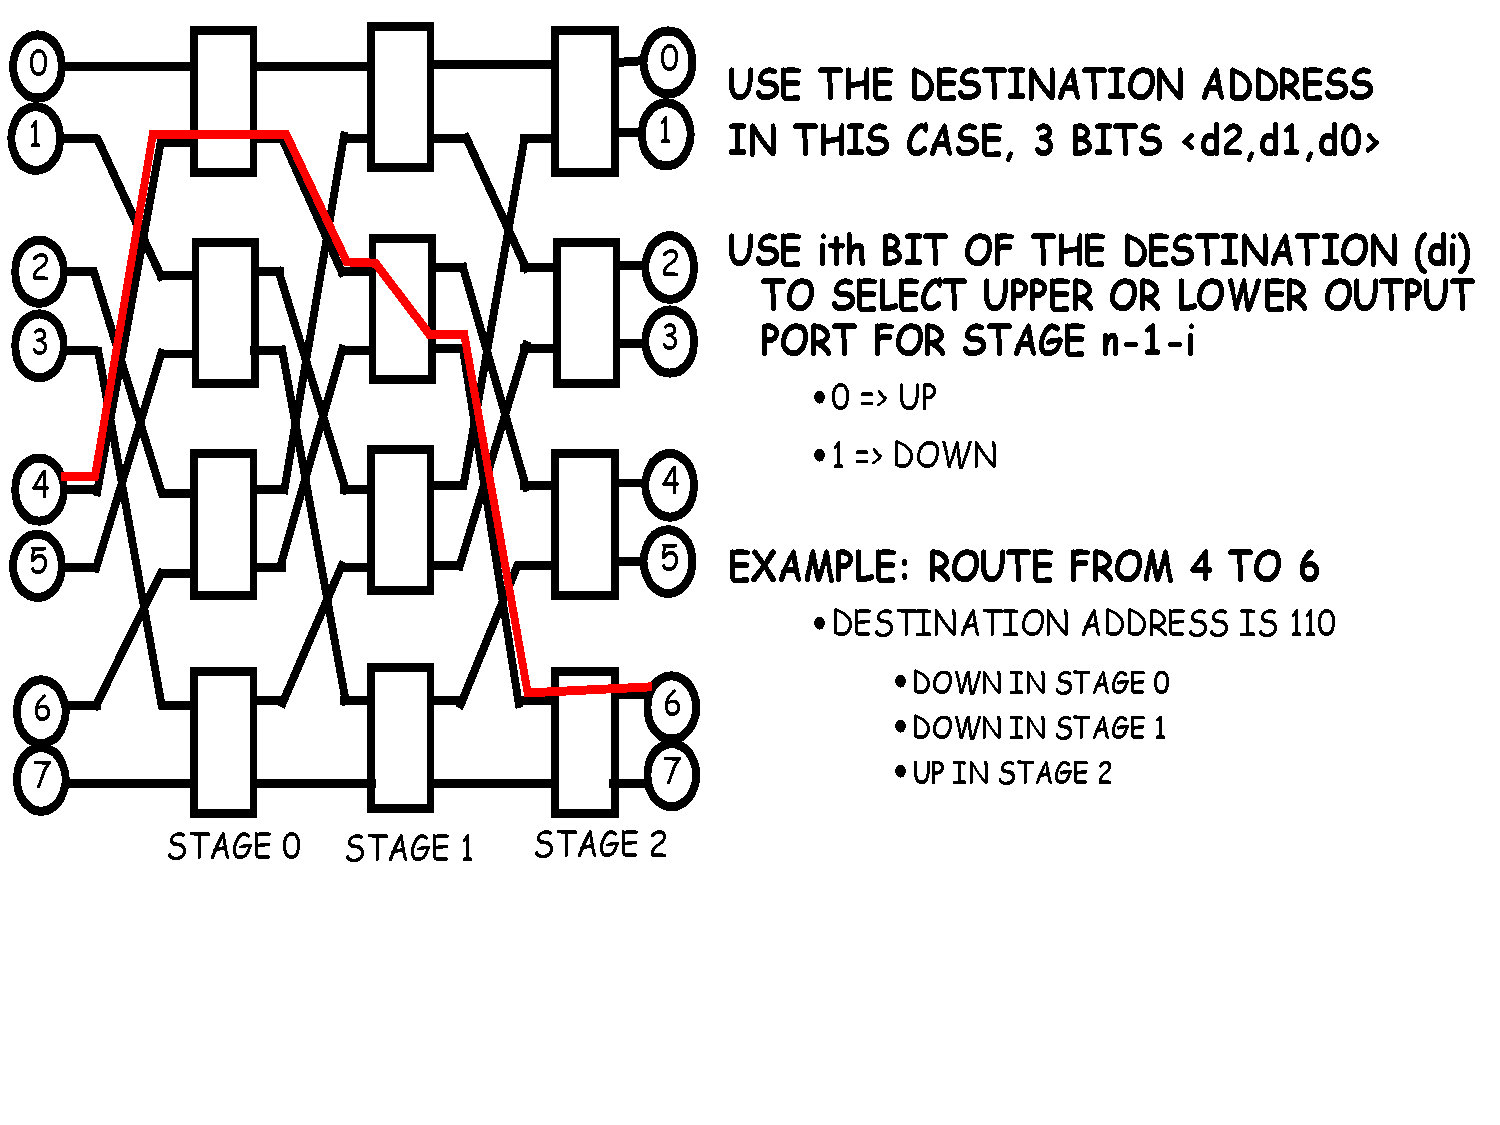
\includegraphics[width=59ex]{FigsInterconnect/OmegaRouting}}

\end{frame}

\begin{frame}[fragile,t]
\frametitle{Routing Algorithm for Butterfly Network}

\emph{Routing Algorithms}: use source/destination address, \emph{are very simple} $\Rightarrow$ 
keep latency small. (Table driven approaches are prohibitive.)

\center{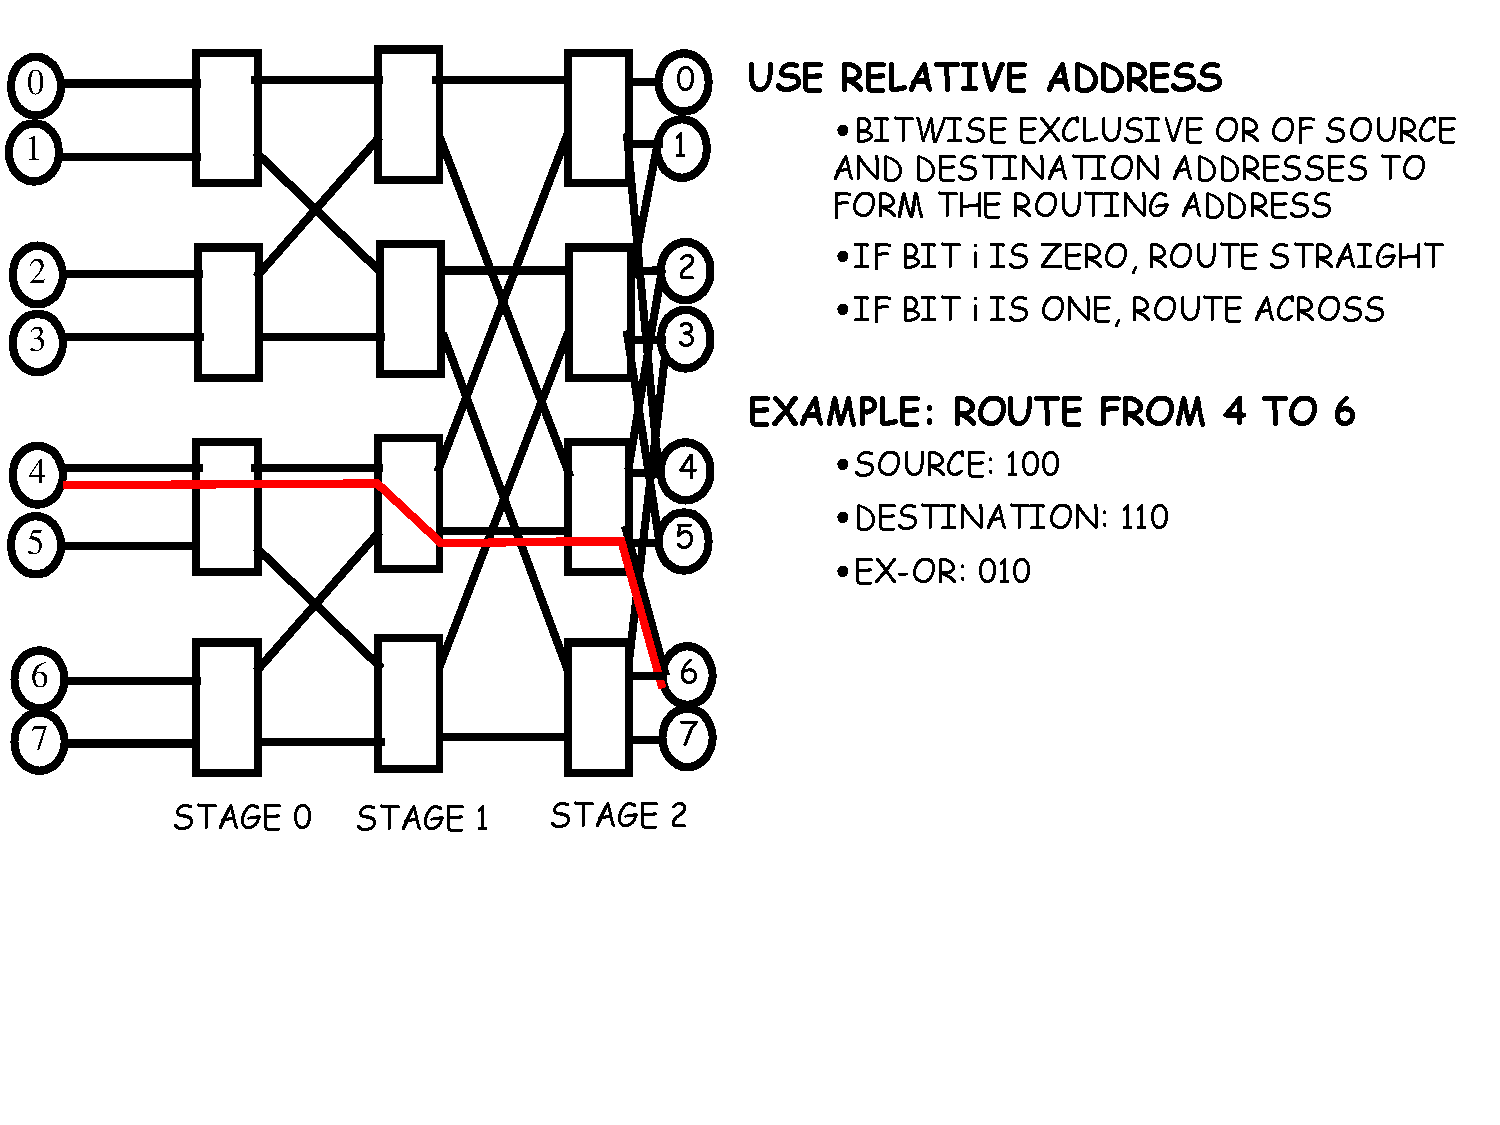
\includegraphics[width=59ex]{FigsInterconnect/ButterflyRouting}}

\end{frame}

\begin{frame}[fragile,t]
\frametitle{Routing Algorithm for Mesh Network}

Dimension-order routing (deterministic). 
\vspace{-3ex}
\center{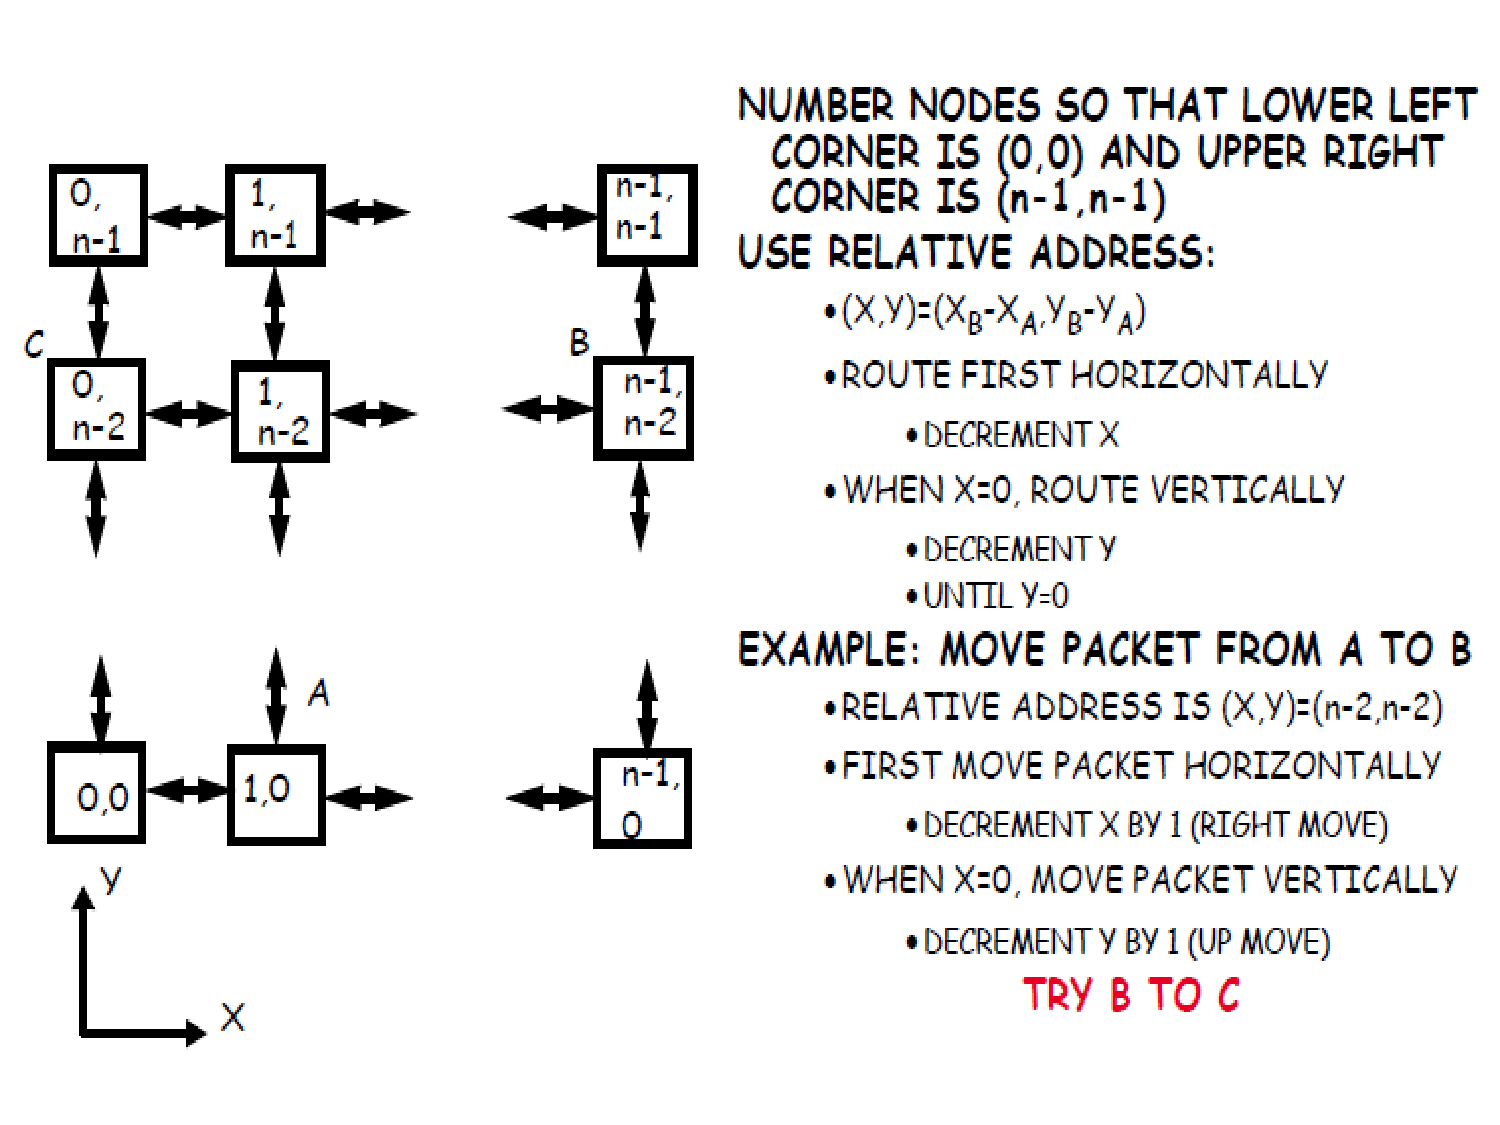
\includegraphics[width=55ex]{FigsInterconnect/DimOrderRouting}}

\vspace{-3ex}
\emp{Hypercube:} XOR (bit-wise exclusive OR) the source and destination address,
            then route in the order of non-zero dimensions. 

\end{frame}



\begin{frame}[fragile,t]
\frametitle{Necessary Conditions for Deadlock}

Assume a set of Agents accessing a Set of Resources.

\begin{itemize}
    \item \emp{Four Necessary Conditions For Deadlock see OpSys:}
    \begin{itemize}
        \item[1] \emp{Mutual Exclusion}: only one agent can access the resource at a time
        \item[2] \emp{No Preemption}: once an agent acquired a resource, no mechanism can force
                it to relinquish it.
        \item[3] \emp{Hold \& Wait}: agent holds acquired resources while waiting for others.
        \item[4] \emp{Circular Wait}: a set of agents wait on each other to acquire other's 
                resources and no one can make any progress. 
    \end  {itemize}\bigskip

%    \item \emp{Shared Resources}: software or hardware, e.g., critical section, disk, printer.
    \item \emph{In Network Case: agents are packets, resources are physical or logical channels.}
\end  {itemize}

\center{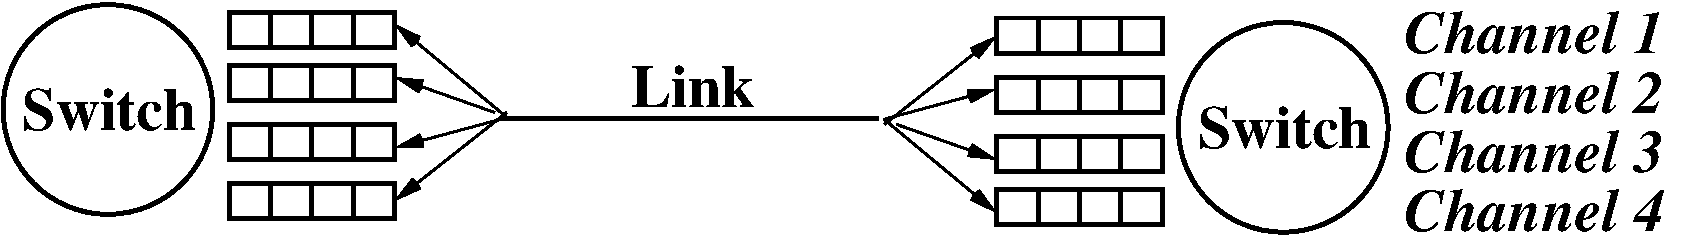
\includegraphics[width=59ex]{FigsInterconnect/Chanels}}

\end{frame}

\begin{frame}[fragile,t]
\frametitle{Deadlock Detection for Mesh and Tori}

\alert{Assume that packets are free to follow any route.}
\medskip

\begin{columns}
\column{0.65\textwidth}
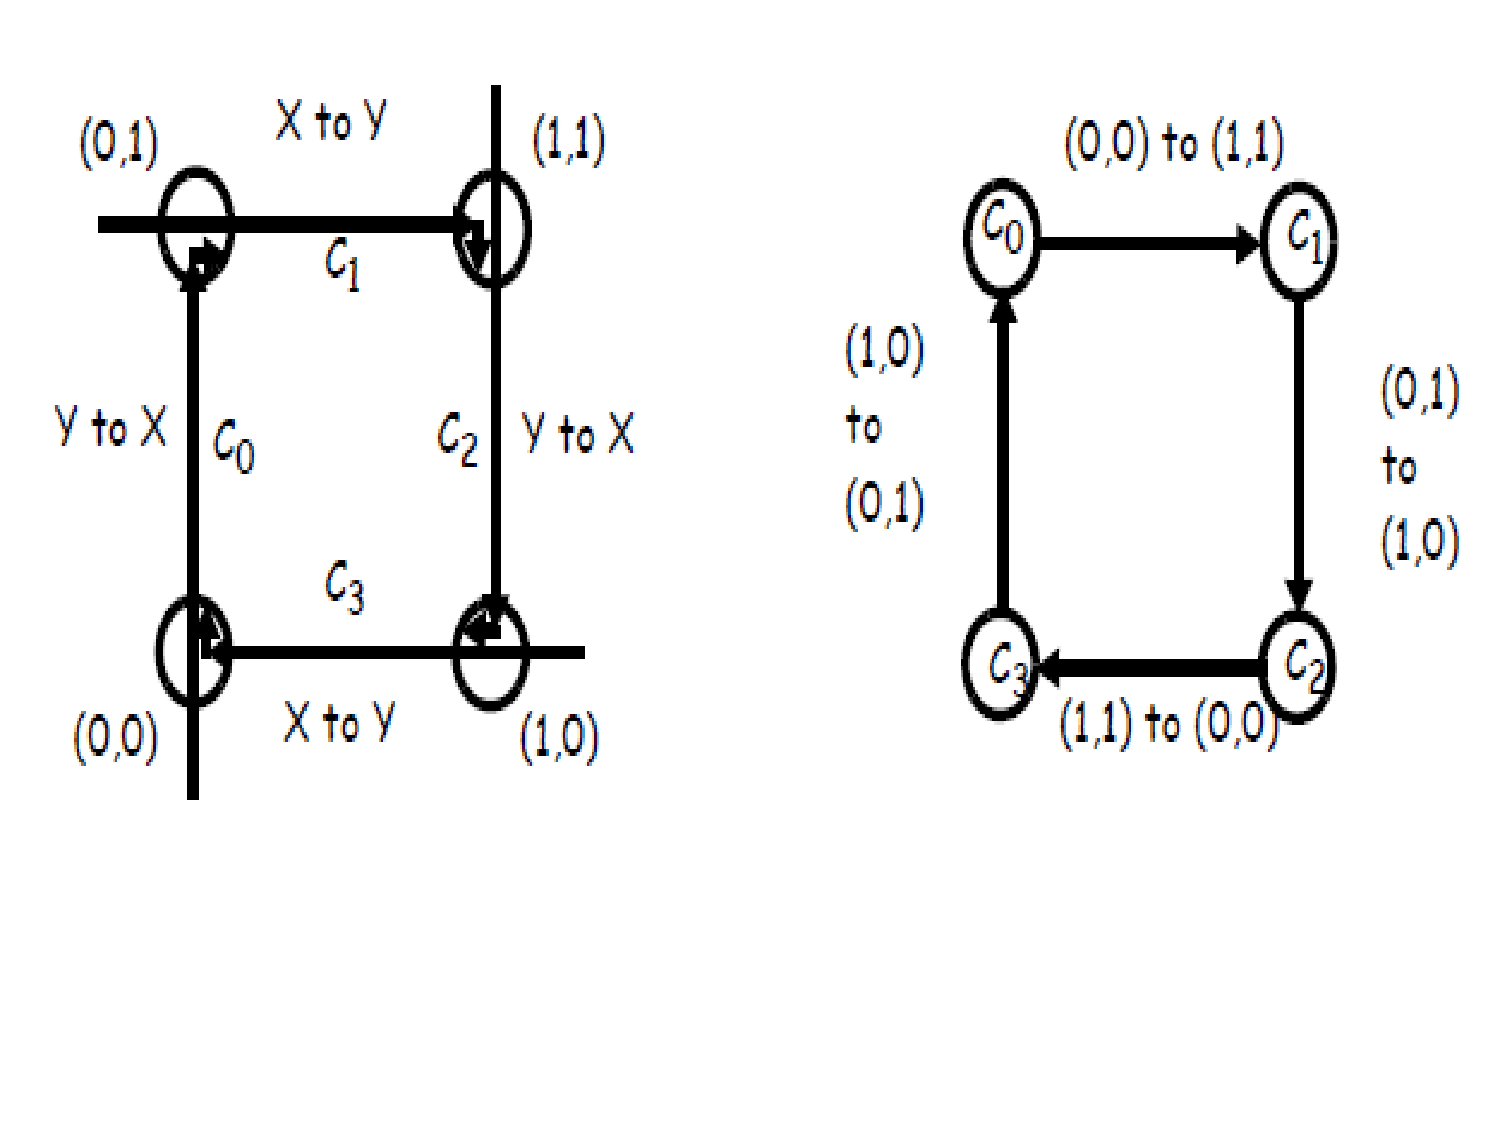
\includegraphics[width=44ex]{FigsInterconnect/DeadlockAvoid1}
\column{0.37\textwidth}
%\begin{scriptsize}
Each node tries in the same time to send 
a packet to the diagonally opposite node, 
e.g., {\tt(0,0}) sends to {\tt(1,1)}.
\medskip

To avoid conflicts {\tt(1,0)} uses first $c_3$ then $c_0$, 
{\tt(0,0)} uses $c_0$ and $c_1$, etc.\\{\tt~~}\\{\tt~~}\\{\tt~~}
%\end{scriptsize}
\end{columns}
\vspace{-5ex}

The Resource Acquisition Graph or \emp{Channel-Dependency Graph}
on the right \alert{has cycles}, hence circular wait, and as such 
\alert{deadlock is possible}.

\end{frame}


\begin{frame}[fragile,t]
\frametitle{Deadlock Avoidance for Mesh and Tori}

\centering{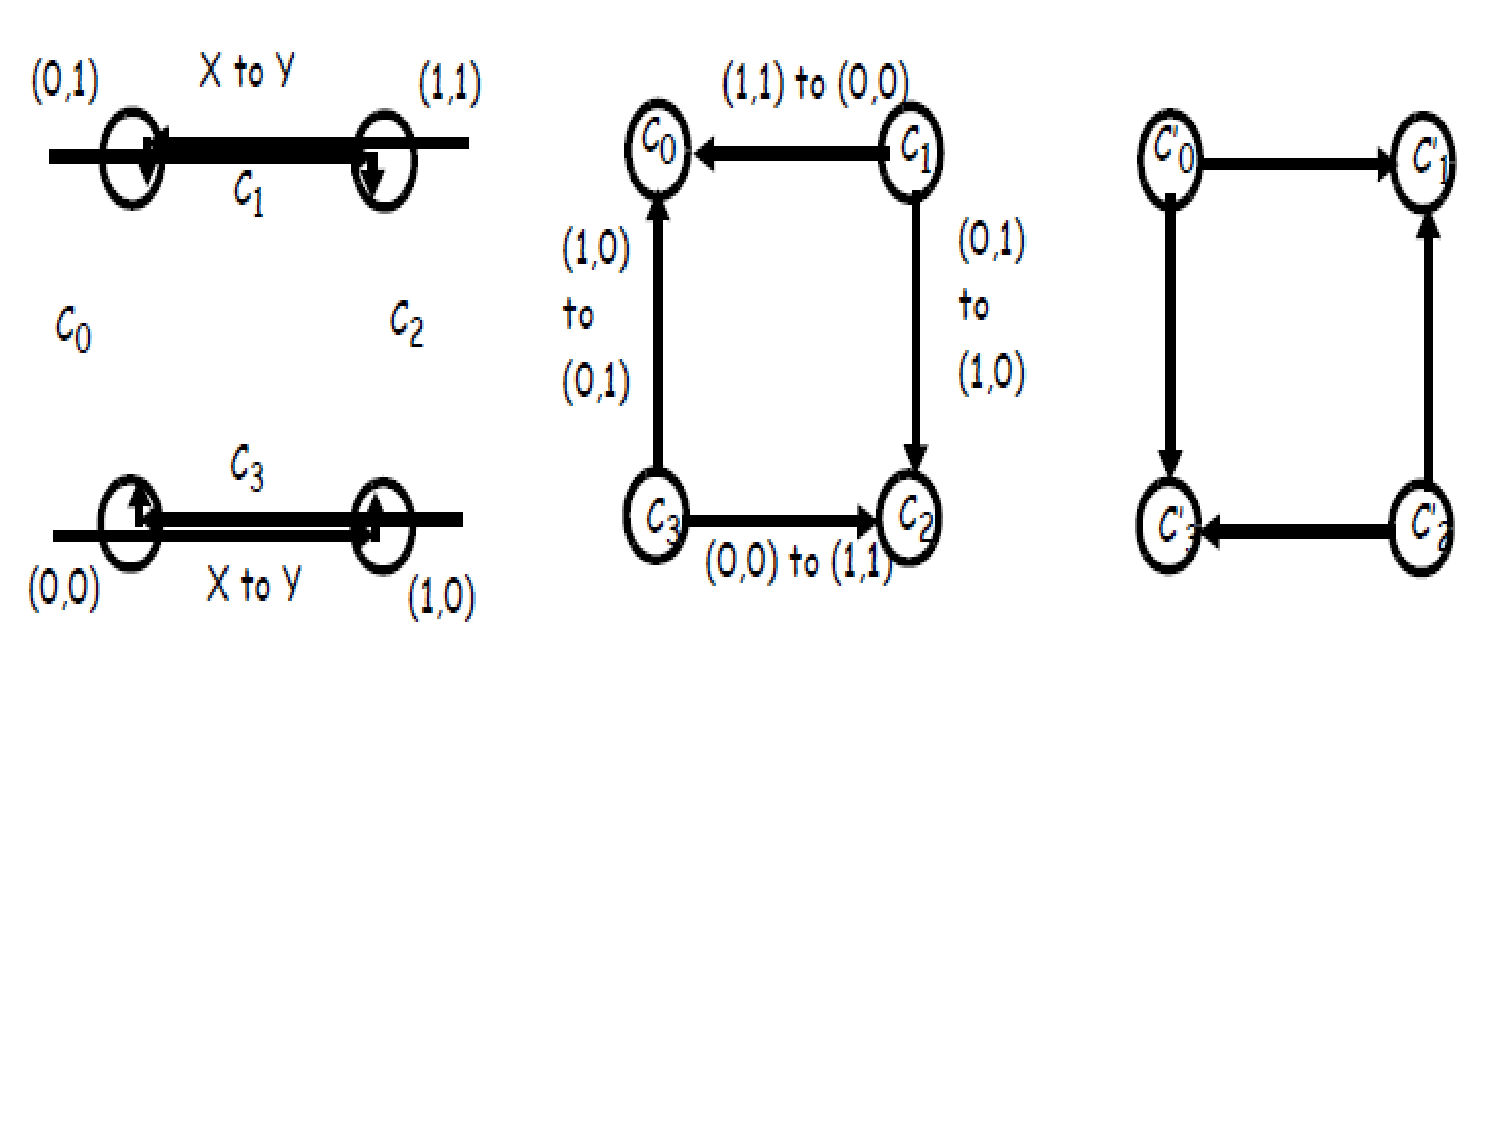
\includegraphics[width=50ex]{FigsInterconnect/DeadlockAvoid2}}
\vspace{-18ex}

\begin{itemize}
    \item \emp{Enforce Dimension Order Routing (XY Routing)}
    \begin{itemize}
        \item Packets move first Horizontally until they cannot anymore,
        \item Then they move Vertically $\Rightarrow$ \emph{No CYCLE, NO DEADLOCK}.
    \end  {itemize}\medskip

    \item \emp{Problem: Contention for Channels $\Rightarrow$ Wasted Bandwidth}
    \begin{itemize}
%        \item If {\tt (0,0)} wants to send a packet to {\tt(1,1)} it must first use $c_3$,
%        \item If $c_3$ is occupied it is still desirable to use $c_0$, but deadlock (?)
        \item \emph{Use virtual channels to increase routing flexibility \& NO deadlock}:
        \item 2 buffers/switch $\Rightarrow$ 2 sets of channels. One uses {\tt XY}, the other {\tt YX}.
        \item Changing at most once from XY to YX routing $\Rightarrow$ NO deadlock.
        \item \emp{\em West-First Routing:} packet is routed in the westward direction if
                destination node is west of source \& NO deadlock.
                \emph{More flexible: only 2 turns are prohibited} (in comparison to 4 for XY).  
    \end  {itemize}\medskip

\end  {itemize}


\end{frame}
\end{document}
